\documentclass[article,type=msc,11pt,colorback,accentcolor=tud9c]{tudthesis}
\usepackage[english]{babel}
\usepackage{titlesec}
\usepackage{natbib}
\bibliographystyle{acl_natbib}
%\setcitestyle{authoryear,open={((},close={))}}
\setcounter{secnumdepth}{4}
\usepackage{acronym}
\usepackage{multirow}
\usepackage{booktabs,tabularx}
\usepackage{placeins}
\usepackage{graphicx}
\usepackage{etoolbox}
\usepackage{setspace} 
\AtBeginEnvironment{quote}{\singlespacing\normalfont}
\usepackage{amsmath}
\usepackage{hyperref}
\usepackage{wrapfig}

\titleformat{\paragraph}
{\normalfont\normalsize\bfseries}{\theparagraph}{1em}{}
\titlespacing*{\paragraph}
{0pt}{3.25ex plus 1ex minus .2ex}{1.5ex plus .2ex}
\newcommand{\getmydate}{%
  \ifcase\month%
    \or Januar\or Februar\or M\"arz%
    \or April\or Mai\or Juni\or Juli%
    \or August\or September\or Oktober%
    \or November\or Dezember%
  \fi\ \number\year%
}

\newcommand{\mx}[1]{\textcolor{red}{max: #1}}

\newcommand{\specialcell}[2][c]{%
  \begin{tabular}[#1]{@{}l@{}}#2\end{tabular}}

\newcommand{\specialcellc}[2][c]{%
  \begin{tabular}[#1]{@{}c@{}}#2\end{tabular}}

\setinstitutionlogo{UKP_logo}

\begin{document}
  \thesistitle{Understanding and Improving Neural Models for Natural Language Interference using External Resources}%
    {Verständnis und Verbesserung Neuronaler Modelle für Natural languge inference}
  \author{Max Glockner}
  \referee{Prof. Dr. Iryna Gurevych}{Andreas R\"ucklé}[Dr.-Ing. Andreas Hanselowski]
  \department{Fachbereich Physik}
  \group{Institut f"ur Angewandte Festkernphysik\\Speerspitze der Elite}
  %\dateofexam{\today}{\today}
  %\tuprints{2616926}{2616926}
  \makethesistitle
  \affidavit{Max Glockner}

\section*{Abstract}
\addtocounter{section}{0}
In recent years, neural approaches relying on distributed word-representations reached state-of-the-art performances on many tasks of Natural Language Processing. Even though these representations lack many information that is present within lexical resources, most neural models to date neglect these resources. In this work we analyse one specific model for the task of Natural Language Inference, in order to identify ways to incorporate lexical semantic relations from WordNet. We exploit the max-pooling mechanism, used to generate the fixed length sentence representations, to identify what information is encoded by the model, how this is done and how the identified encoding scheme can finally be used to derive the prediction label. Even though the high performance of neural networks for Natural Language Inference suggests, that this task is well understood, we show by creating an additional testset, derived from the trainset, that several state-of-the-art models can easily be failed with simple lexical inferences. Doing so, we show that the performance does not stem from a good Natural Language Understanding but relies on dataset-specific pattern, indicating the need to infer this information from external resources. We target this problem by inferring WordNet information by either concatenating new word-vectors to the orignal word-representations, or by changing sentence-representations, based on this information, using multitask-learning. While both experiments do not yield any improvements, we identify the need to include external information in a general and easy-to-exploit way for the network, in order to overcome problems from dominant arbitrary dataset-specific patterns and enable the generalization of specific word-relations, even if some are not directly used within the train data.
\newpage\cleardoublepage
\section*{Zusammenfassung}
In den letzten Jahren erreichten neuronale Netzwerke State-of-the-Art Ergebnisse in vielen Bereichen von Natural Language Processing, indem sie ausschließlich auf Informationen aus kontextbezogenen Wortrepräsentationen zurückgreifen. Obwohl diese Repräsentationen ein Defizit an vielen Informationen aufweisen, die in lexikalischen Ressourcen verfügbar sind, werden diese Ressourcen weitgehend bei neuronalen Ansätzen ignoriert. In dieser Arbeit widmen wir uns der Analyse eines speziellen Models für Natural Language Inference, mit dem Ziel, Strategien zu identifizieren, lexikalisch-semantische Beziehungen aus WordNet zu integrieren. Hierzu nutzen wir den max-pooling Mechanismus aus, der verwendet wird, um Vektorrepräsentationen fester Länge für Sätze zu erstellen. Somit untersuchen wir, welche Informationen vom Model enkodiert werden, wie dies getan wird und wie diese Art von Kodierung zur Herleitung der Klassifizierung genutzt werden kann. Obwohl die starken Ergebnisse neuronaler Netze für Natural Language Inference nahelegen, dass dieser Bereich  weitgehend gelöst ist, zeigen wir mithilfe eines neuen Testsets, basierend auf den Trainingsdaten, dass einfache lexikalische Schlussfolgerungen bereits große Probleme für State-of-the-Art Modelle darstellen.  Wir zeigen somit, dass die guten Ergebnisse nicht Folge eines stabilen Sprachverständnisses der Models sind, sondern Folge der Ausnutzung diverser häufig auftretender Muster im Datensatz sind, und die Integration dieser Informationen relevant für die Verbesserung ist. Wir versuchen das Problem zu lösen, indem wir zusätzliche Informationen den Wortrepräsentationen anhängen oder die Satzrepräsentationen basierend auf jenen Informationen mithile von Multitask-Learning anzupassen. Beide Experimente resultieren nicht in der gewünschten Verbesserung. Jedoch idenifizieren wir den Bedarf, externe Informationen möglichst allgemeingültig zu integrieren, sodass diese einfach vom Model erkannt und genutzt werden könnwn. So kann das neuronale Netzwerk das Problem dominanter datensatzspezifischer Muster überkommen, und über Wortrelationen generalisieren, ohne, dass jede einzelne direkt in den Trainingsdaten verwendet werden muss.
\addtocounter{section}{0}

\newpage\cleardoublepage
\section*{List of abbreviations}
\addtocounter{section}{0}

\begin{acronym}[Bash]
 \acro{biLSTM}{bidirectional Long-Short-Term Memory Network}
 \acro{BoW}{Bag of Words}
 \acro{ESIM}{Enhanced Sequential Inference Model}
 \acro{HIT}{Human Intelligence Task}
 \acro{IE}{Information Extraction}
 \acro{IR}{Information Retrieval}
 \acro{KIM}{Knowledge-based Inference Model}
 \acro{LSTM}{Long-Short-Term-Memory}
 \acro{MLP}{Multi Layer Perceptron}
 \acro{MSE}{Mean Squared Error}
 \acro{MultiNLI}{MultiGenre Natural Language Inference Corpus}
 \acro{NLI}{Natural Language Inference}
 \acro{NLP}{Natural Language Processing}
 \acro{NLU}{Natural Language Understanding}
 \acro{POS}{Part of Speech}
 \acro{OANC}{Open American National Corpus}
 \acro{QA}{Question Answering}
 \acro{ReLU}{Rectified Linear Units}
 \acro{RNN}{Recurrent Neural Network}
 \acro{RTE}{Recognizing Textual Entailment}
 \acro{SD}{Standard Deviation}
 \acro{SICK}{Sentences Involving Compositional Knowledge}
 \acro{SNLI}{The Stanford Natural Language Inference Corpus}
 \acro{WSD}{Word Sense Disambiguation}
 \acro{YAGO}{Yet Another Great Ontology}


\end{acronym}
\newpage\cleardoublepage
\tableofcontents
\newpage\cleardoublepage
\section{Introduction}
In recent years neural networks again gained a lot of popularity for many machine learning tasks, including the field of \ac{NLP}. While previous generation solutions heavily depended on handcrafted features, these models are capable of learning meaningful feature representations automatically \citep{bengio2013representation}, thus avoiding the time consuming process of feature-engineering. For the most part, neural networks solely rely on distributed word representations, like word2vec \citep{mikolov2013distributed} or GloVe \citep{pennington2014glove} and typically learn fixed-length dense vector representations for the input text. While those distributed word-vectors provide strong generalization capabilities, they fail to capture simple world-knowledge \citep{celikyilmaz2010enriching} and even have trouble differentiating between mutually exclusive words, if they generally are used in similar contexts \citep{vulic2017morph}. As opposed to neural models relying on distributed representations, traditional approaches execively made use of lexical resources containing relational and factual information about words and entities. Despite being well studied and containing valuabe information that is not present within distributed word-vectors, those lexical resources are for the most part ignored by neural approaches. Intuitively, combining the approaches with complementary strengths, the generalization power of distributed representations and the knowledge-rich structures of lexical resources, may further lead to better \ac{NLU} capabilities of models and thus increase the performance on a wide variety of tasks.

\subsection{Goal of this thesis}
The goal of this work is to identify directions to incorporate this external knowledge into neural models. This is highly aligned with the way, humans understand text, by having a solid understanding of the world, that influences the subjective interpretation of every word within a sentence. Given the sentence ``The official language in the USA is English.'' an average human can conclude that the official language of ``New York'' also is English, knowing that ``New York'' is within the ``USA''. We try to solve this problem on the task of \ac{NLI} \citep{bowman2015large}, also known as \ac{RTE} \citep{dagan2006pascal}. As this is known to be a fundamental task for \ac{NLU} \citep{maccartney2007natural}, insights gained here can improve other tasks of \ac{NLP} that indirectly depend on it. Specifically, we try to incorporate external knowledge into the sentence-representation of a state-of-the-art model for \ac{NLI}. Therefore, we start by analysing how sentences are encoded within that model, identifying the role of different dimensions and how the encoded values within those dimensions serve the final prediction. To show the relevance of the knowledge we infer, we create an additional test-set for \ac{NLI}, that can be considered to be easily solvable based on the train-data, if the predictions indeed are based on a proper \ac{NLU}. On this new dataset we finally evaluate two strategies to infer the required knowledge, either by adding it to the word-representations or, by fusing it into the sentence representation.

\subsection{Structure of this thesis}
While we explain relevant techniques and concepts, we expect the reader to have a basic understanding of common machine-learning practices, neural networks (including basic network architectures like \ac{LSTM} or \ac{RNN}) and \ac{NLP} in general. Opinions expressed within the thesis are those of the author and may not necessarily correspond to the opinions of other participators, even though everything is expressed using ``we''. In some sections, especially with mathematical equations, we assign meanings to single symbols, written in italic like $p$ or $h$. Unless we specifically mention that those will be identical for the remainder of the full thesis, we may re-define the meaning of those symbols in later sections. The code for all experiments is available on github\footnote{\href{https://github.com/Max216/ThesisPKinDL}{https://github.com/Max216/ThesisPKinDL}}.
\newline

\noindent
We give a quick overview of the content within this thesis:
\begin{itemize}
\item Section §\ref{sec:basics} introduces the task of \ac{NLI} as well as the state-of-the-art model we use throughout most of the experiments. Additionally, lexical semantic relations, which play a crucial role for this work, are defined.
\item In Section §\ref{sec:related_work} we introduce relevant datasets for \ac{NLI} and discuss several neural approaches, proved to be successful. In addition, we show and describe lexical resources, that contain relevant information to improve the \ac{NLU} of neural models, as well as various strategies that have been applied to integrate them.
\item We analyse how the information of a natural language text is encoded within the sentence representation of a neural model and give insights on how the model uses it in Section §\ref{sec:understanding}.
\item We derive a new testset from a major dataset for \ac{NLI}, demonstrating the poor generalization abilities of state-of-the-art models without external knowledge in Section §\ref{sec:additional_snli_set}.
\item Based on the new testset, we evaluate strategies to incorporate external knowledge into the sentence-representations, by either fusing the knowledge with the word-representations or directly into the sentence-representations using multitask-learning in Section §\ref{sec:approaches_ext_res}.
\end{itemize}\newpage\cleardoublepage
\section{Theoretical Background}\label{sec:basics}
This section gives an overview of the task that is used within this work (§\ref{sec:basics_nli}) and relevant datasets regarding this task (§\ref{sec:basics_datasets}).
\subsection{Natural Language Inference}\label{sec:basics_nli}
\ac{NLI} \citep{bowman2015large} deals with the problem to identify, whether one piece of natural text, namely the \textit{hypothesis}, can be inferred from another piece of text, namely the \textit{premise}. The hypothesis $h$ is said to be entailed by the premise $p$ if a human reader would conclude that the hypothesis is true, given the fact that the premise is true. Therefore it differes from strict logical inference. While in \ac{NLI} a high plausability for the premise to imply the hyothesis, based on the human judgement, is sufficient, the latter one strives to achieve certainity \citep{dagan2009recognizing}. \ac{NLI} essentially breaks down to an alignment problem \citep{maccartney2008phrase}. Given the sentence pair
\begin{center}
\begin{tabular}{rl}
\textbf{Premise:} & \textit{Donald Trump is eating his cheeseburger in his bedroom.} \\
\textbf{Hypothesis:} & \textit{The president of the United States is snacking a cheeseburger in the White House.} 
\end{tabular}
\end{center}
the model is required to correctly align \textit{Donald Trump} with \textit{The president of the United States}, \textit{eating} with \textit{snacking} and have information that his \textit{bedroom} is within the \textit{White House}. Here it can be seen, how the system would not only need to cope with different ways of expressing the same meaning, due to the nature of language, but also is required to access and process factual information, that is commonly known to an average human. 
\newline
\subsubsection*{Relatedness to other NLP tasks}
While \ac{NLI} clearly is central to reasoning capabilities, it is very fundamental and applicable to a large variety of \ac{NLP} as the ability to recognize textual entailment is a fundamental and necessary problem towards real \ac{NLU} \citep{maccartney2007natural,bos2005recognising}. Many \ac{NLP} applications such as \ac{QA}, Summarization \ac{IE} implicitly depend on this ability, as the huge variability of possible expressions for the same meaning it is a core phenomen of natural language \citep{dagan2009recognizing}. All three tasks require the model to infer that the target meaning of interest can be inferred from any other variant of textual expression. For \ac{QA} it is the identification of a correct answer, for summarization, the complete summary needs to be implied by the original text and similarily, while redundant sentences expressing the same meaning should be ommited. Similarily \ac{IE}, especially if using multiple documents, needs to infer, whether two variants of text contain the same information. Even simple paraphrasing can be broken down to a lexical inference problem with mutual entailment between $p$ and $h$. As end applications for \ac{NLP} in addition to \ac{NLU} need to solve another complicated machine-learning task it is hard to compare and directly improve their \ac{NLU} capabilities. Thus, one of the main purposes of \ac{NLI}, being a very basic problem towards \ac{NLU}, serves a a benchmark  with any improvements helping a large variety of high level tasks \citep{williams2017broad,cooper1996using,bos2005recognising,dagan2006pascal}. 

\subsection{Lexical Semantic Relations}\label{sec:word_relations}
\mx{TODO: lexical inference \citep{shwartz2015learning} and being the semantic relation between two terms (bi/unidirectional)}
Lexical relations describe the relationship between words\footnote{While there is no single definition for \textit{word}, we refer assume a single word to have the same surface form and the same lemma.} whereas \textit{Lexical Semantic Relations} specifically indicate relations referring to the meaning of the word. \citep{murphy2003semantic} and have shown to be helpful for detecting lexical inferences \citep{dagan2009recognizing}. We define the following relations based on those of \cite{Jurafsky2008May}. One key characteristic of natural language is ambiguity, tht is also present in lexical semantics as words may have several meanings or \textit{senses}\footnote{The phenomen of words having multiple senses is called \textit{homonymy}, if both senses show indicate no relation but share the surface form like ``bank'' (financial institution) and ``bank'' (sloping mound). If those senses are semantically related like ``milk'' (take milk from female mammals) and ``milk'' (like cow's milk), the relationship is called \textit{polysemy} \citep{Jurafsky2008May}}. To deal with this phenomene, lexical semantic relations are defined between senses rather than words. For the sake of simplicity for the most part we follow a naive approach in the following chapters of assuming the most dominant sense of a word, when referring to it. Specifically we define \textit{Synonymy}, \textit{Antonomy}, \textit{Hypernomy} and \textit{Holonomy}, the latter two relations are visualized\footnote{This is for illustration purposes only and we only added some relevant relations between the entities, more relation are possible. For instance, the holonym relationship would of course hold between \textit{head} and any other \textit{animal}.} in Figure \ref{fig:lexical_resources}.
\begin{figure}[tph!]
\centering
	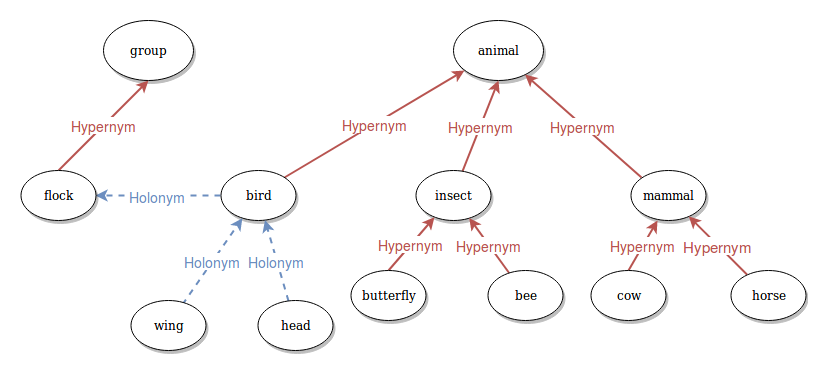
\includegraphics[totalheight=7cm]{fig/lexical_relations.png}
	\caption{A sample ontology of animals to illustrate the lexical relations \textit{Hypernomy} and \textit{Holonymy}.}
	\label{fig:lexical_resources}
\end{figure}
\subsubsection{Synonymy and antonomy}
Synonomy is a symmetric relationship between two senses or two words. Two senses of two different words are said to be synonyms, if they have the same or nearly the same meaning. Synonymy between words is holds, if one word can be replaced by the other word in any sentence  without changing the meaning of the sentence. True synonyms are rare, as most words at least have subtle differences in their meaning or are used within different contexts. We thus follow common practice and loosen the strict definition by refering to synonmys if they have approximately similar meanings. Like synonomy, antomy is a symmetric relationship between senses, however having the opposite meaning, which might be caused by a binary opposition like ``opened/closed'', by different ends on some scale like ``hot/cold'' or by directional change like ``upwards/downwards''. Since antonyms semantically are identical in all other aspects with synonyms, these relations are hard to distinguish from each other automatically.

\subsubsection{Hypernomy}
Hypernomy (or Hyponomy) is an asymmetric relation between two senses and also referred to as the \textbf{is-a} relation. The more specific sense (e.g. \textit{bee}) is called a hyponym of the more general sense (e.g. \textit{insect}), which is called hypernym. \cite{Jurafsky2008May} give a formal definition for Hyponomy in terms of entailment: 
\begin{quotation}\noindent
``[...] a sense $A$ is a hyponym of a sense $B$ if everything that is $A$ is also $B$ and hence being an $A$ entails being a $B$, or $\forall x$ $A(x) \Rightarrow B(x)$.'' \citep{Jurafsky2008May}
\end{quotation}
Hypernomy is in most casses transitiv, thus if a \textit{cow} is hyponym of \textit{mammal} and \textit{mammal} is a hyponym of \textit{animal}, \textit{cow} is also a hyponym of \textit{animal}. an important phenomen for this thesis are two words, sharing a close hypernyms. In Figure \ref{fig:lexical_resources}, \textit{bee} and \textit{butterfly} share the hypernym \textit{insect}, we refer to them as co-hyponyms.

\subsubsection{Holonomy}
Holonomy or Meronomy refers to the \textbf{part-whole} relation. In the illustration of Figure \ref{fig:lexical_resources}, the \textit{wing} is a part of a \textit{bird} and a \textit{bird} is a part of a \textit{flock}. We say that a \textit{bird} is a meronym of \textit{flock}, while \textit{flock} is the holonym of \textit{bird}. As opposed to Hypernyomy, this asymmetric relation is not automatically transitiv. While a \textit{flock}\footnote{This is an example for polysemy, as \textit{flock} may refer to a group of birds, but also to a group of e.g. sheep. In this case we assume the sense of a group of birds.} obviously consists of several birds, In this case \textit{birds} is generally not replacable with \textit{heads}. 

\subsection{Shortcut-Stacked-Encoder and Residual Encoder}\label{sec:residual_encoder_def}
We conducted most of our experiments with the Shortcut-Stacked-Encoder \citep{nie2017shortcut} and the recently adapted version to the Residual Encoder for \ac{NLI}. They achieve state-of-the-art results\footnote{Considering models for SNLI without inter-sentence attention.} for two large datasets\footnote{These are explained in detail in §\ref{sec:basics_datasets}} for \ac{NLI} and follow the Siamese Architeture, originally introduced by \cite{bromley1994signature}, thus first encoding $p$ and $h$ using the same sentence encoder with shared weights into fixed length sentence representations and then predicting the entailment label from the combination of both representations using an additional \ac{MLP}.

\subsubsection{Sentence Encoding for Shortcut-Stacked-Encoder}
The key novelty of this approach is the way sentence representations are created using a three-layer \ac{biLSTM} with shortcut connections and row-wise max-pooling. An overview of this architecture is given in Figure \ref{fig:sentence_emcoder_shortcut}.
\begin{figure}[tph!]
\centering
	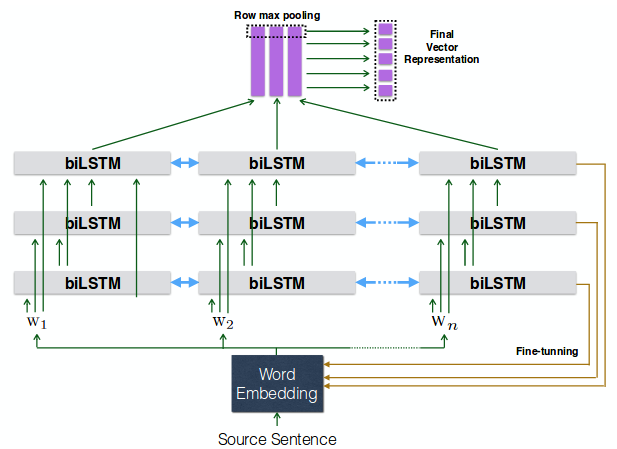
\includegraphics[totalheight=8cm]{fig/sentence_encoder_shortcut.png}
	\caption{The architecture of the sentence-encoding component within the Shortcut-Stacked-Encoder, taken from \cite{nie2017shortcut}.}
	\label{fig:sentence_emcoder_shortcut}
\end{figure}
Due to the arbitrary length of words in textual input a widely used strategy to encode variable length inputs to fixed length vectors using \ac{LSTM} \citep{hochreiter1997long} or the bidirectional variant \ac{biLSTM} \citep{graves2005framewise}. Essentially these components learn with the use of gates what information to keep and forget at a given point in time. By sequentially going through a sentence in one or two directions respectivly, are capable of exploiting word-order and take context into account.
\newline

The main difference of the Shortcut-Stacked Sentence-Encoder to typical approaches of a multi-layer \ac{biLSTM} model is that the input to the \ac{biLSTM} in a following layer is not only the output of the previous layer, but the output of \textit{all} previous layers, together with the word embeddings. In the first step, the embedding layer maps each word $\omega_i$ of the source sentence $(\omega_1, \omega_2, ..., \omega_n)$ to a $d$-dimensional word vector $w_i \in \mathbb{R}^d$. According to \cite{nie2017shortcut} we denote $x_t^i$ to be the input of the $i$th \ac{biLSTM} at timestep $t$. Naturally the input to the first layer are the word-embeddings itself, thus:
\begin{equation}
x_t^1 = w_t
\end{equation} 
In all \ac{biLSTM} with $i > 1$ the input is the concatenation of all intermediate inputs of previous layers at the timestep $t$ together with the initial word embeddings. Let $[]$ denote the vector concatenation and $h^i_t$ be the output of the $i$th \ac{biLSTM} at timestep $t$, this leads to:
\begin{equation}\label{eq:stacked_encoder_input}
x_t^i = [w_t, h_t^{i-1}, h_t^{i-2}, ... , h_t^1]
\end{equation}

Only the last \ac{biLSTM} layer is used to generate the final sentence representation. Assuming $m$ layers in total, $d_m$ to be the hidden state dimension of the last layer, that is defined as $H_m=(h_1^m, h_2^m, ..., h_n^m)$ the final sentence representation $v$ is obtained by applying row-max-ppoling over the last layer:
\begin{equation}
v = max(H^m)
\end{equation}
With each $h_i^m \in \mathbb{R}^{2d_m}$ and $H^m \in \mathbb{R}^{2d_m \times n}$ the resulting sentence vector $v \in \mathbb{R}^{2d_m}$ essentiallly captures the highest value of each dimension over all timesteps\footnote{$d_m$ is multiplicated by $2$ since the \ac{biLSTM} creates $d_m$ features for going through the sentence forwards and backwards repsectively.}.
\subsubsection{Classification}
A two-layer \ac{MLP} using ReLu as acticvation function and a final softmax-layer is used for the prediction. The input to the classifier $m$ is the concatention of the sentence representations $v_p$ and $v_h$ for $p$ and $h$ respectively together with the element-wise distance and the elementwise product, denoted as $\otimes$ of both representations:
\begin{equation}
m = [v_p, v_h, |v_p-v_h|, v_p \otimes v_h]
\end{equation}
Even thow a multi-layer \ac{MLP} theoretically would be able to learn the latter two features, \cite{mou2015natural} showed that this particular feature concatenation gives a performance gain for neural models for \ac{NLI}.
\subsubsection{Training}
For all our reimplementations using pytorch\footnote{\href{http://pytorch.org/}{http://pytorch.org/}} of the model we follow the parameters of the original paper of \cite{nie2017shortcut}. The model is trained using Adam \citep{kingma2014adam} parameter optimization, cross-entropy loss as objective function and minibatches of size 32. To avoid overfitting a dropout of 0.1 is applied on each layer of the \ac{MLP} and the accuracy is evaluated regulary on a different dataset than the train data, the development set, as it is common practive in machine learning. The final performance is estimated by evaluating the best model based on the accuracy on the development set on unseen hold-out data, the test set. 300-dimensional GloVe 840B pretrained word-embeddings \citep{pennington2014glove} are used and finetuned during training. Three additional word-vectors are added, one for unknown words, as well as one to indicate the start and one to indicate the end of a sentence. The learning rate starts with 0.0002 and is reduced by half every second iteration. We conduct our experiments with different re-implementations of this model, partly due to using fewer parameters by reducing the dimensionality of the components, partly due to changes within the original paper.
\subsubsection{Residual Encoder and Reimplementation Variants}
In a second version of the paper, \cite{nie2017shortcut} introduced the Residual Encoder, slightly adapting the way sentences are encoded. In order to create the input to the $i$th \ac{biLSTM} layer $x_t^i$ concatenation all previous outputs $(h_t^{i-1}, h_t^{i-2}, ... , h_t^1)$ together with $w_t$, naturally leads to a tremendous increase of parameters. By using residual connections, instead of concatenating all previous outputs, they are added up, thus equation (\ref{eq:stacked_encoder_input}) changes to
\begin{equation}
x_t^i = [w_t, h_t^{i-1} + h_t^{i-2} + ... + h_t^1]
\end{equation}
and reduces the parameter size.
\paragraph*{Implementation Variants}
We use the following implementations of the model. The performance comparison between the models based on SNLI\footnote{SNLI is a huge dataset for \ac{NLI} and will be explained in §\ref{sec:basics_datasets}}, is listed in Table \ref{table:reimplementation_performance} and do not differ tremendously from what \cite{gong2017natural} estimated to be the human performance on the same task.
\begin{table}[!htbp]
\begin{center}
\begin{tabular}{lccc}
\textbf{Model} & \textbf{SNLI train acc.} & \textbf{SNLI dev acc.} & \textbf{SNLI test acc.}\\
\toprule
Shortcut-Stacked Encoder\textsuperscript{$\dagger$} & 87.4\% & 85.2\% & 84.8\% \\
Shortcut-Stacked Encoder\textsuperscript{$\dagger\dagger$} & 89.4\% & 86.0\% & 85.4\% \\
Residual Encoder\textsuperscript{$\dagger$} & 91.1\% & 85.9\% & 85.8\% \\
Residual Encoder\textsuperscript{$\Diamond$} & 91.0\% & 87.0\% & 86.0\% \\
\midrule
Human Performance \citep{gong2017natural} & - & - & 87.7 \\
\bottomrule
\end{tabular}
\caption{Accuracy in percent of different implementations of the model from \cite{nie2017shortcut}, achieved on the SNLI dataset compared with human performance.}
\label{table:reimplementation_performance}
\end{center}
\end{table}
\begin{itemize}
\item We refer to Shortcut-Stacked Encoder\textsuperscript{$\dagger$} as the first re-implementation. This uses $256\times2$, $512\times2$ and $1024\times2$ dimensions for the three layers of the sentence encoding \ac{biLSTM} and $1600$ dimensions in the classifier \ac{MLP}.
\item We refer to Residual Encoder\textsuperscript{$\dagger$} when we use our own re-implementation with residual connections. The sentence-encoding \ac{biLSTM}s each have the dimensionality of $600\times2$ and the layers of the \ac{MLP} of $800$.
\item We refer to Residual Encoder\textsuperscript{$\Diamond$} when we use the final published version of \cite{nie2017shortcut} with their provided code\footnote{https://github.com/easonnie/ResEncoder}. This model has the same parameter sizes as Residual Encoder\textsuperscript{$\dagger$}.
\item We refer to the plain model name, when talking about the model structure in general.
\end{itemize}
\newpage\cleardoublepage
\section{Related Work}\label{sec:related_work}
Much work has been done to create strong models for \ac{NLI} and we show some successful strategies in Section §\ref{sec:models_snli}. Relevant datasets for \ac{NLI} are introduced in Section §\ref{sec:basics_datasets}. Before the excessive usage of neural networks, many models heavily relied on external resources, that have either been manually created in order to improve tools for \ac{NLP}, or arised in a crowd sourced manner for a different purpose, but can also be exploited. In Section §\ref{sec:ext_resources} we show an overview of some external resources that might improve the performance of neural models on \ac{NLI}. While most neural models rely solely on distributed word-representations as external information and perform quite good, prior work \citep{bos2005recognising,tatu2005semantic} depended to large degree on those resources. In Section §\ref{sec:ext_res_in_nn} we show several approaches trying to combine the power of well structured, knowledge-rich resources with the generalization power, coming from neural models with distributed word embeddings.
\subsection{External Resources}\label{sec:ext_resources}
A large variety of knowledge bases exist, containing for instance lexical relations or commonly known world knowledge, which can be helpful for improving the performance on \ac{NLI}. Research has shown that both, manually created and crowd-sourced resources, can successfully be applied in many tasks of \ac{NLP}. In this section we only show WordNet and Wikipedia, containing different information that we consider to be useful for \ac{NLI} and \ac{NLU}, as well as two resources combining multiple resources and thus providing a huge amount of readily-available knowledge.

\subsubsection{WordNet}\label{sec:wordnet}
\begin{wrapfigure}[13]{R}{0.5\textwidth}
\centering
	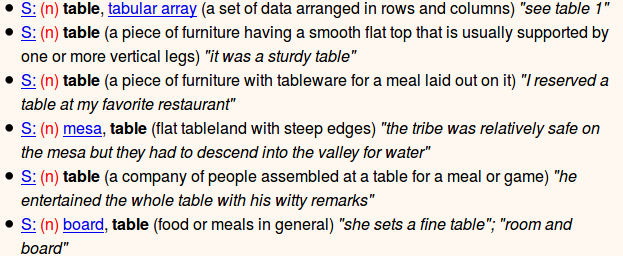
\includegraphics[totalheight=3.5cm]{fig/wordnet_example.png}
	\caption{Example of different synsets of the lemma ``table'' (only noun senses) within WordNet, taken from \href{http://wordnetweb.princeton.edu}{http://wordnetweb.princeton.edu}.}
	\label{fig:wordnet}
\end{wrapfigure}
WordNet \citep{miller1995wordnet} is a famous, manually created lexical resource for the English language consisting of thre lexica for four different \ac{POS}, one for verbs, one for nouns and one for adjectives and adverbs respectively \citep{Jurafsky2008May}. 
\paragraph*{Structure of WordNet} 
Mainly focusing on nouns\footnote{WordNet 3.0 contains 117,798 nouns, 11,529 verbs, 22,479 adjectives and 4,481 adverbs \citep{Jurafsky2008May}.} it differentiates between the more frequent class of \textit{common nouns} like ``table'' and \textit{instances} like ``Berlin''. All words are represented by their lemma and due to polysemy contain one or more senses, namely \textit{synsets}. Synsets are the main building blocks within the WordNet ontology, containing a sense description and examples. Figure \ref{fig:wordnet} displays 6 different senses for the lemma ``table''. It is noteworthy that the sense of table (as tabular array) greatly differs from the sense as ``furniture'' or ``tablelands'' while metaphorical senses strongly correlate with the sense of table as a furniture. Yet, they encode much more fine-grained sense-differences, that differ only slightly from each other, compared with the difference in meaning off the first synsets. While lemmata within the same synset refer to the lexical semantic relation synonymy, other lexical semantic relations like hypernomy, antonomy and holonomy (as described in Section \ref{sec:word_relations}, however more fine-grained\footnote{For example,  WordNet differentiates between \textit{hypernyms} for common nouns and \textit{instance-hypernyms} for instances, or distinguished between \textit{part- }, \textit{member-} and \textit{substance-holonyms}.} within WordNet) are defined via labelled links between synsets. Thus, WordNet holds valuable knowldge for detecting lexical inferences in natural language.

\paragraph*{Usage and Issues}
When using WordNet in applications one has to identify the correct sense out of many possible synsets for a given lemma. This may be done using proper algorithms for \ac{WSD}. Another simple and frequently used heuristic is to always choose the first snyset, which typically reflects the most common sense \citep{mccarthy2004using}. As shown in Figure \ref{fig:wordnet}, word-senses are defined with different granularities, sometimes varying only with subtle differences that are not required by most applications. Subsequently, this reduces the interpretability of path lengths of lexical relations between two synsets. For instance, identifying that ``sunflower'' is a hyponym of ``plant'' requires the traversal over five edges (\textit{sunflower $\rightarrow$ flower $\rightarrow$ angiosperm $\rightarrow$ spermatophyte $\rightarrow$ vascular plant $\rightarrow$ plant}). At the same time, identifying that a ``church'' is a ``building'' can be identified by only traversing over two edges (\textit{church $\rightarrow$ place of worship $\rightarrow$ building}) and traversing similarily over five edges leads to the synset ``whole, unit'', covering both, living things and objects. This is a known issue \citep{resnik1995using} and  strategies have been proposed to reduce the complexity of WordNet, if the specific domain is known, for instance using sense clustering \citep{prakash2007learning}.

\subsubsection{Wikipedia}\label{sec:wikipedia}
While WordNet contains manually annotated lexical relations and is easily and automatically accessable, Wikipedia\footnote{\href{https://www.wikipedia.org/}{https://www.wikipedia.org/}} is a huge multi-lingual, continuously growing  encyclopedia, maintained by many volunteers. Also mostly focusing on nouns, due to the nature of containing ecyclopedic information, it contains a large variety of factual information about named entities, that many other lexical resources lack \citep{gurevych2016linked}. Even though it has not been created for the purpose of serving as a lexical knowledge base, it still may be seen as  partially annotated resource, due to artifacts like hyperlinks. These can be interpreted similarily and even accessed using available tools in a programmatic manner \citep{zesch2008extracting}.  \cite{gurevych2016linked} describe the following information types that can be exploited to retrieve lexical information:
\begin{itemize}
\item \textbf{First paragraph:} The first paragraph of an article can be interpreted as the \textit{sense definition}, since every article covers only one aspect due to the nature of encyclopedias.
\item \textbf{Hyperlinks:} \textit{Sense examples} can be retrieved from the context, surrounding a hyperlink that links to the entity of interest, showing how the term is used.
\item \textbf{Hyperlinks:} Hyperlinks between articles can be considered as \textit{sense relations}.
\item \textbf{Translation Pages:} Due to interlinked articles in different languages, the corresponding titles usually can serve as \textit{translation equivalents}.
\end{itemize}
Wikipedia has successfully been used in many applications for \ac{NLP} and even though we do not conduct experiments within this work using Wikipedia, it clearly contains rich factual and world knowledge that can be helpful for \ac{NLI} systems. 
\subsubsection{Derived from multiple Knowledge Bases}
\ac{YAGO} \citep{suchanek2007yago} combines the high coverage of Wikipedia with the clean taxonomy of WordNet, leading to a very knowledge rich resource. \ac{YAGO} mainly targets to contain a large amount of world-knowledge with Wikipedia, as being tremendously larger than WordNet, and additionally contains relations to express facts derived from it. As opposed to \ac{YAGO}, UBY \citep{gurevych2012uby} aims for lexical semantic richness. In addition to Wikipedia and WordNet, seven other resources are combined together, providing lexical semantic knowledge in German and English. The combination is realized by using so-called \textit{sense axis}, links between two senses of different lexicons. UBY provides an easy-to-use API, making its high-coverage knowledge programatically accessable to \ac{NLP} applications. Having these knowledge-rich resources available, but for the most part de-coupled from neural approaches, still lacking this exact knowledge, stresses the benefit of combining these two worlds. 

\subsection{Datasets for NLI}\label{sec:basics_datasets}
As neural models usually require a huge amount of data for their training, they were not successfully applicable to \ac{NLI} tasks until the release of \ac{SNLI}, where they reach state-of-the-art results. Previous \ac{NLI} tasks like FraCas \citep{cooper1996using} or the PASCAL challenge \citep{dagan2006pascal} only consisted of a very limited amount of training data, such that neural models could not be used successfully. Some datasets, like \ac{SICK} \citep{marelli2014semeval} or the Denotation Graph entailment set \citep{young2014image}, increased the amount of samples at the expense of using artificially created sentences and/or automatically labeling, reducing the textual quality and adding noise. Since the focus in this work is on neural models, only the relevant datasets for this purpose are introduced.
\subsubsection{SNLI}\label{sec:snli}
With the release of \ac{SNLI} \citep{bowman2015large} researchers were able to apply neural models for the task of \ac{NLI} using distributed word. The corpus consists of 570,152 human written sentence pairs and differentiates between the three labels, described in Section §\ref{sec:basics_nli}. 
\paragraph*{Event co-reference}
A drawback of all previsously existing resources for \ac{NLI}, that is handled by \cite{bowman2015large}, is the fact that even humans may assign different labels to a sentence pair, based on their subjective interpretation of a sentence, that all can be valid. This issue can be demonstrated using the following sentence pair:
\begin{center}
\begin{tabular}{rl}
\textbf{Premise:} & Young people are demonstrating in San Francisco.
\\
\textbf{Hypothesis:} & Young people are demonstrating in New York.
\end{tabular}
\end{center}
One could clearly argue the sentence-pair should be labelled as \textit{neutral}, since there could be people demonstrating in both towns. However it is also legimate to interpret these as contradicting sentences, if one considers both sentences to be describing the same event. While both sentences may be true when describing different potential scenarios, only one of them can be true if they refer to the same. In order to reduce noise coming from these inconsistent interpretations, the labeling scheme within \ac{SNLI} must be fixed beforehand. Specifically they choose the labelling scheme to be based on event-coreference, the latter of the two explanations, as otherwise only very general statements would result in \textit{contradiction}.
\paragraph*{Generation}
In order to create \ac{SNLI}, \cite{bowman2015large} used image captions from the Flickr30k corpus \citep{young2014image} as premises and let human workers create according hypothesis for each label respectively using Amazon Mechanical Turk by asking them to write alternative captions that
\begin{itemize}
\item definetely also are a true description of the photo  \textbf{(entailment)}
\item might be a true description of the photo \textbf{(neutral)}
\item definetely are a false description of the photo \textbf{(contradiction)}
\end{itemize}
The workers only saw the image caption, not the image itself, but were encouraged to use common world knowledge, enabling the creation of inferences that require additional information of the world, that is not available in word-embeddings\footnote{For instance (taken from \ac{SNLI}) \textit{snow} is paraphrased as \textit{frozen particles of water} and requires very deep factual knowledge to be understood correctly.}. While this process simplifies the task of assuming event-coreference, the sentences within \ac{SNLI} are rather simple and short, due to the nature of image captions. 

\paragraph*{Looking into data}
As we conduct most of the experiments of this work on \ac{SNLI}, it is important to get an understanding how sentences in this dataset look like. As previously mentioned, the vast majority of sentences are rather simple and might even be phrases only, rather than proper sentences, due to omission of a verb. In addition to that, sentences might be written in proper English, but also might contain spelling or punctuation errors, be lowercased only, or describe highly unrealistic scenarios.  Table \ref{table:snli_example} shows selected sample sentence-pairs, taken from the \ac{SNLI} dataset.
\begin{center}
\begin{table}[htt]
\begin{center}
\resizebox{\textwidth}{!}{%
\begin{tabular}{lll}
\textbf{Premise} & \textbf{Hypothesis} & \textbf{Label} \\
\toprule
\multirow{3}{*}{\textbf{(1)} The large brown dog jumps into a pond.} & The dog is getting wet. & \textit{entailment} \\ & The dog is a chocolate Labrador Retriever. & \textit{neutral} \\
&A white cat is sunning itself on a windowsill. & \textit{contradiction} \\
\midrule
\multirow{3}{*}{\textbf{(2)} A woman is handing out fruit.} & A woman is passing out different types of fruits. & \textit{entailment} \\
&A woman is handing out oranges. & \textit{neutral} \\
&A fruit is handing out a woman. & \textit{contradiction} \\
\midrule
\multirow{3}{*}{\textbf{(3)} A basketball game.} & A sports game. & \textit{entailment} \\
&A basketball game between rivals. & \textit{neutral} \\
&A volleyball game. & \textit{contradiction} \\
\bottomrule
\end{tabular}}
\end{center}
\caption{Example sentence pairs, taken from \ac{SNLI}, showing typical sentences within the dataset.}
\label{table:snli_example}
\end{table}
\end{center}
The first column displays the premise, the original image caption, in the second column three hypothesis are shown, created by the workers for each label respectively. Several characteristics of the dataset and types of required knowledge to solve the task can be seen here. 
The first examples \textbf{(1)} require the model to have some factual knowledge that a ``Labrador Retriever'' is some kind of ``dog'', and ``chocolate'' is paraphrasing ``brown''. Since ``Labrador Retriever'' is a possible substitute for ``dog'' but more specific, the sample is labelled as neutral. The according entailing hypothesis requires an even deeper understanding of the world, as the system needs to know, that a ``pond'' is filled with water and anything that goes into water is ``getting wet''. The contradicting sample shows two frequently occuring characteristics. Not only has ``dog'' been replaced by ``cat'', but also the color and the activity changed. We found that in many contradicting hypothesis several contradicting words with respect to the premise exist, obviously making the task easier, as it is sufficient to only detect one several indicators. Additionally it has been shown that the creation process of the hypothesis followed some unconscious heuristics of the worker\citep{gururangan2018annotation}. Specifically the replacement of ``dog'' to ``cat'' occurs often enough, that the presence of ``cat'' in the hypothesis alone is a strong indicator for contradiction already. 
\newline

\noindent
The sentences of the second example \textbf{(2)} are based on paraphrasing, representing the same meaning, (entailment), have more specific term in the hypothesis as in the premise (neutral) and show semantic role reversal (contradiction),  which is somewhat interesting, as it requires to model to leverage word order, while a simple \ac{BoW} approach would fail here.
\newline

\noindent
In contrast to \textbf{(1)} the sentences in \textbf{(3)} only require very shallow knowledge. Here, the word ``basketball'' is substituted by it's hypernym\footnote{At least in one sense, not in the sense of \textit{being a ball}.} ``sport'', thus still covering the original meaning by being more general. The next sentence gives some plausible additional information not given in the premise, hence neutral. In the last contradicting sentence, the model has to identify that ``basketball'' and ``volleyball'' are mutually exclusive, which shows, how co-hyponyms influence the relation label. While sentences are often a bit longer than in this example, the required knowledge, as specified in \textbf{(3)}, is most present within \ac{SNLI}.

\subsubsection{MultiNLI}
\ac{SNLI} received some critizism within the research community \citep{chatzikyriakidis2017overview,williams2017broad}, mainly due to it's simplicity, cominng from the fact, that all premises are taken from a single genre only, namely image captions. Thus, \ac{SNLI} is very limited to only visual scenes, neglecting many other aspects like temporal reasoning, modality or belief. \cite{williams2017broad} introduced with \ac{MultiNLI} a new dataset, overcoming these drawbacks. 
\paragraph*{Generation of \ac{MultiNLI}}
The authors followed the same generation procedure as has been done by \cite{bowman2015large}, but instead of relying on image captions only, they took into considerations other genres from \ac{OANC}\footnote{Genres from \ac{OANC}: \textit{Government, Slate, Telephone Speech, Travel Guides, 9/11 Report, Face-to-face Speech, Letters, Nonfiction Books, Magazine}} \citep{ide2001american,ide2004american,ide2006integrating} as well as several freely available fiction work, resulting in 10 additional genres with 392,702 new sentence-pairs for training and 20,000 for development and test respectively. A major motivation for the creation of \ac{MultiNLI} was, to put more emphasis on the role of \ac{NLI} as evaluation benchmark of \ac{NLU} that \ac{SNLI} failed to provide due to its narrow coverage. Therefore, only five of the new genres are present within the train data, while the remaining five genres only occur in the test set, serving as evaluation for cross-domain transfer learning and domain adaption. The performance on this dataset is measured in two figures, \textit{matched} examples are derived from the same source as training samples, while \textit{mismatched} examples differ from those seen during the training (containing the additional genres). This motivation becomes also clear from the corresponding Shared Task \citep{nangia2017repeval}, allowing any kind of external resources (including the ones that were used to derive the premises) but only accepting sentence-encoding models\footnote{These models encode each sentence individually and are explained in Section §\ref{sec:models_snli}.} to evaluate sentence representations learning with respect to \ac{NLU}. \ac{MultiNLI} has been shown to be harder than \ac{SNLI} \citep{williams2017broad}, the best performing model of the RepEval 2017 Shared Task reaches 74.9\% matched and mismatched accuracy \citep{chen2017recurrent} using ensembles and 74.5\% matched, 73.5\% mismatched accuracy using a single model\citep{nie2017shortcut}. 
\paragraph*{Looking into data}
Table \ref{table:multinli_example} depicts a few samples of different genres\footnote{Taken from https://repeval2017.github.io/shared/}. One can see how different genres broaden the scope of language that is used to express inferences. A system needs to deal with temporal information and less visualizable terms like \textit{appreciate} or \textit{benefit}.
\begin{center}
\begin{table}[h]
\begin{center}
\resizebox{\textwidth}{!}{%
\begin{tabular}{llll}
\textbf{Premise} & \textbf{Hypothesis} & \textbf{Label}  & \textbf{Genre} \\
\toprule
\multirow{3}{*}{\parbox{6cm}{The Old One always comforted Ca'daan, except today.}} & \multirow{3}{*}{\parbox{6cm}{Ca'daan knew the Old One very well.}} & & \\
& & \textit{neutral} & Fiction \\
& & & \\
\midrule
\multirow{3}{*}{\parbox{6cm}{Your gift is appreciated by each and every student who will benefit from your generosity.}} & \multirow{3}{*}{\parbox{6cm}{Hundreds of students will benefit from your generosity.}} & &\\
&  & \textit{neutral} & Letters \\
& & & \\
\midrule
\multirow{3}{*}{\parbox{6cm}{At the other end of Pennsylvania Avenue, people began to line up for a White House tour.}} & \multirow{3}{*}{\parbox{6cm}{People formed a line at the end of Pennsylvania Avenue.}} &  & \\
& & \textit{contradiction} & 9/11 Report \\
& & & \\

\bottomrule
\end{tabular}}
\end{center}
\caption{Example sentence pairs from \ac{MultiNLI}, taken from RepEval 2017 Shared Task, showing samples of different genres.}
\label{table:multinli_example}
\end{table}
\end{center}
As the authors followed the same guidelines, as used for \ac{SNLI}, and also assume event-coreference, both datasets are highly compatible, only differing in the range of genres and thus diversity of language. In fact, \ac{MultiNLI} is even distributed in the same data format and a common practive is, to include data from \ac{SNLI} when training models for \ac{MultiNLI} \citep{nie2017shortcut,balazs2017refining,yang2017character}.

\subsubsection{SciTail}
SciTail \citep{scitail} is yet another dataset for \ac{NLI}, designed to address a different problem of previously existing datasets\footnote{Ignoring small-scale datasets with less than 1,000 samples.}. The targeted problem of previous work, including \ac{SNLI}, is, that either the premise or the hypothesis was specifically for this task created, thus neglecting the kind of naturally occuring inference problems of any endtask like \ac{QA}. It is comparably smaller, consisting of only 27,026 examples and only distinguishes between two labels, \textit{entailment} and \textit{neutral}. \textit{Entailment} is defined as in \ac{SNLI} and \ac{MultiNLI}, saying that the premise supports the hypothesis. All cases where the hypothesis is not supported by the premise however are classified \textit{neutral}.

\paragraph*{Generation of SciTail}
In order to retrieve premise and hypothesis from a resource, rather than creating one sentence for the specific purpose of \ac{NLI}, \cite{scitail} took a different approach to generate the corpus. The dataset originates from school-level multiple-choice questions for science \ac{QA} \citep{welbl2017crowdsourcing}. Those questions generally require sophisitcated reasoning capabilities in order to answer them correctly. 
\begin{enumerate}
\item \textbf{Hypothesis:} Given the short factual answer-candidates and a question, a new sentence was synthesized using the question and answer. This sentence serves as the hypothesis. For instance the question ``When waves of two different frequen-
cies interfere, \textit{what phenomenon occurs?}'' and the orrect answer ``beating'' is transformed into ``When waves of two different frequencies interfere, \textit{beating occurs}'' \citep{scitail}.
\item \textbf{Premise:} A large background corpus with relevant information from \cite{clark2016combining} was used to generate candidate knowledge sentences for each question using \ac{IR} for the premise.
\item \textbf{Label:} While hypothesis, derived from an incorrect answer, can be assumed to be not-supported by the premise, those derived from a correct answer are not necessarily supported by the sentence gained from the background corpus (the premise). Thus, samples where croud-sourced annotated, to ensure a correct labelling, only keekping those samples as entailment, that were labelled to have \textit{Complete Support}\footnote{Annotators could decide between \textit{Complete support} (labelled as entailment), \textit{Partial Support} (ignored) and \textit{Unrelated} (labelled as neutral).}.
\end{enumerate}


\paragraph*{Comparison with \ac{SNLI} and \ac{MultiNLI}}
Due to it's design, SciTail is different in nature to the two previous datasets. Neither does it contain contradicting examples, nor does assume event-coreference, as sentence-pairs in this dataset are more based on factual information. Table \ref{table:scitail_example} shows somple sentences of the SciTail dataset. Clearly all of them contain factual information, whereas in the previous shown datasets, sentences tend to be more situational. The premise can be relevant for the entailment relation, yet must not be. 
\begin{table}[!htbp]
\begin{center}
\begin{tabular}{lll}
\textbf{Premise} & \textbf{Hypothesis} & \textbf{Label} \\
\toprule
\multirow{3}{*}{\parbox{9cm}{Bones come together to form joints, most of which are in constant motion.}} & \multirow{3}{*}{\parbox{5cm}{Joints are the location where bones come together.}} & \multirow{3}{*}{\parbox{2cm}{\textit{entailment}}}\\
& &  \\
& &  \\
\multirow{4}{*}{\parbox{9cm}{Bone, Joint, and Muscle Disorders Chapter 54 Charcot's Joints Charcot's joints (neuropathic joint disease) results from nerve damage that impairs a person's ability to perceive pain coming from a joint;}} & \multirow{4}{*}{\parbox{5cm}{Joints are the location where bones come together.}} & \multirow{4}{*}{\parbox{1.5cm}{\textit{neutral}}}\\ 
& &  \\
& &  \\
& &  \\
\midrule
\multirow{3}{*}{\parbox{9cm}{The time to travel the horizontal distance (the range) is equal to twice the time to reach the peak (maximum height).}} & \multirow{3}{*}{\parbox{5cm}{Range is the maximum horizontal distance traveled by a projectile.}} & \multirow{3}{*}{\parbox{1.5cm}{\textit{entailment}}}\\
& &  \\
& &  \\
\multirow{3}{*}{\parbox{9cm}{First, finding the launch angle for maximum horizontal range in idealized projectile motion.}} & \multirow{3}{*}{\parbox{5cm}{Range is the maximum horizontal distance traveled by a projectile.}} & \multirow{3}{*}{\parbox{1.5cm}{\textit{neutral}}}\\ 
& &  \\
& &  \\
\bottomrule
\end{tabular}
\caption{Example sentence pairs from SciTail Task, different premises retrieved for two hypothesis.}
\label{table:scitail_example}
\end{center}
\end{table}
Due to its relatedness with Scientific \ac{QA}, the authors claim, that a model reaching a good performance on this dataset for \ac{NLI} will also score well on an according \ac{QA} task, as similar \ac{NLU} is needed.
\subsection{Neural Models for NLI}\label{sec:models_snli}
We follow the \ac{SNLI} leaderboard\footnote{https://nlp.stanford.edu/projects/snli/} by differentiating between \textit{sentence-encoding} and \textit{inter-sentence-attention} based models. In the following, we show an overview about relevant approaches of both areas. The Residual Encoder or Shortcut-Stacked Encoder, as introduced in Section §\ref{sec:residual_encoder_def}, belongs to the former class of models. 
\subsubsection{Sentence Encoding Models}
Sentence-encoding models follow the Siamese Architecture \citep{bromley1994signature}, meaning they encode both, sentences $p$ and $h$, individually, with parameters being tied between both sentence encoders. The inference classification is predicted by a following classifier like a \ac{MLP}. Doing so, the models put more emphasis on a meaningful sentence representation with the motivation of being more generally applicable and less focused on the specifc characteristics of the task at hand \citep{bowman2016fast}. Many different strategies are used to create meaningful sentence representations within this class of neural models. This is for instance done by exploiting syntactical information using neural Shift-Reduce-Parsers, that create a linear sequential structure from tree-structures sentence representations \citep{bowman2016fast}, or by adding and external memory with read- and write-operations, capturing the temporal and hierarchical information within natural language \citep{munkhdalai2017neural}. 

\paragraph*{Inner-attention-based models}
Following the intuition that humans only remember certain parts of a sentence after reading it, \cite{chen2017recurrent} model this human behaviour using gated intra-sentence attention, by generating the sentence representation via pooling\footnote{As done with max-pooling by \cite{nie2017shortcut}.} strategies over the outputs of the encoding \ac{biLSTM}. The outputs are reweighted using  attention gates. The idea of using inner-attention mechanisms is also used by the best performing sentence encoders for \ac{SNLI}, at the time of this writing reaching 86.3\% in accuracy \citep{shen2018reinforced,im2017distance}. \cite{shen2018reinforced} create sentence representations using the combination of hard and soft self-attention\footnote{A plain attention function calculates the alignment for an input sequence $x=[x_1, x_2, ...,x_n]$ given a query $q$. In the special case of self-attention, $q$ arises from the input sequence $x$ itself \citep{shen2018reinforced}.}. While hard-attention forces the model to only focus on relevant elements of the input sequence, disregarding all other elements, it is not fully differentialbly and thus inefficient to train. Soft-attention methods on the other hand, are fully differentiable and weight each element of the input sequence accoridng to their relevance. However, by also giving positive, non-zero weights to irrelevant elements, it diminishes the emphasis on truely important ones. By first applying hard-attention to retrieve a subset of context-aware elements, that is afterwards processed using soft-attention, \cite{shen2018reinforced} leverage the mentioned advantages both techniques. Inner attention is also used by \cite{im2017distance}, however their model additionally uses directional masks, that prevent the network from considering following or predeeding words in the attiontion proces respectively. Furthermore, they use distance masks, that reduce the attention weights, if words are further away to each other. They show that their model outperforms others, especially with longer input sentences, as the result of considering word distance and positional information.

\subsubsection{Inter-sentence-attention-based models}\label{sec:rel_work_sentence_encoding_models}
\cite{rocktaschel2015reasoning} shows, that models perform significantly better, when looking at both sentences simultaneously in the senteence-encoding step. This is motivated by the way, humans would solve the task of \ac{NLI}, by first reading the premise, and creating the understanding of the hypothesis based on the previously read sentence. Since this seems to be superior in \ac{SNLI}, many works follow this approach reaching state-of-the-art results. Also in this class of methods memory networks, accessable via attention, were applied \citep{cheng2016long}.

\paragraph*{Inter-sentence-attention-based models used within this work}
\cite{parikh2016decomposable} provide a simple network structure, called \textit{Decomposable Attention}, using the assumption that only parts of a sentence are needed for the entailment relationship. They do so by fragmenting the input sentences into subphrases and align the fragments of both sentences with each other using attention. Even though they represent sentences in a \ac{BoW} manner, they reach a remarkable performance. After comparing the aligned phrase-pairs, the final sentence representation is retrieved by a simple summation over the comparison-vectors from the previous step. Thus, by using this rather basic aggregation method rather than relying on any \ac{LSTM}-based method, they reduce computational complexity tremendeously. \ac{ESIM} \citep{chen2017enhanced} is another simple yet strong model, essentially consisting of three different steps. First, words are encoded using \ac{biLSTM}s such that they represent the context as well as the word itself. Next, similarily to \cite{parikh2016decomposable}, they calculate the local inferance between elements in both sentences, by reweighting the sentence representations, based on the normalized attention weights. They enhance this information, using the feature concatenation of \cite{mou2015natural}, as done in the Shortcut-Stacked Encoder, however in this approach word order information is preserved by the network, in contrast to Decomposable Attention. The final sentence representation is created using pooling\footnote{As opposed to summation in Decomposable Attention. \cite{chen2017enhanced} evaluate in their experiments, that pooling leads to superior results than summation, due to being less sensitive to the sentence length.} on the ouput of a \ac{biLSTM}, composing the local inference information from the previous step. The composed vector is finally fed into a \ac{MLP} classifier for the prediction. \cite{chen2017enhanced} report their results using an ensemble of two inplementations with the same base architeccture. One, as described here, relies on a \ac{biLSTM}, the other focuses more on syntactic features by encoding sentences with a TreeLSTM. While Decomposable Attention and ESIM achieve competitive results on \ac{SNLI} we conduct experiments using both models in Section §\ref{sec:additional_snli_set}, showing that these results are rather a matter of memorization than generalization.

\paragraph*{Attempt to incorporate WordNet}
Very recently, \cite{chen2017natural} introduced with \ac{KIM} a neural model, incorporating information from WordNet. This is, at the time of this writing,  the single best performing model on \ac{SNLI}. In their approach, they map WordNet relations, as defined in Section §\ref{sec:word_relations}, to a real number $r \in \mathbb{R}$ with $0 \leq r \leq 1$, quantifying the relations between word within $p$ and $h$ based on the path length of each relation within WordNet, and represent each word-pair with this additional feature vector. However evven by enrichening the representations with WordNet information, they only outperform models without external information by a small margin, ranging from 0.1 to 0.6 points in accuracy. \cite{chen2017natural} show that adding WordNet is helpful if less train data is available, however only show limited evidence, that the model leverages from WordNet fused relations for the overall improvement in accuracy\footnote{This is true for the first published version \citep{chen2017natural}. Subsequentially to work presented within this thesis in Section §\ref{sec:additional_snli_set}, they show indeed that the additional information from WordNet is a key factor within \ac{KIM} in their updated version \citep{chen-EtAl:2017b:natural}.}. In this paper we show that performance on \ac{SNLI} is not sufficient evidence for the capability of dealing with simple lexical inferences as inferred from WordNet, which suggests that further investigations should be conducted in this direction.

\paragraph*{Benchmark}
To this date, the best single sentence-encoding models on \ac{SNLI} reach 88.6\% \citep{chen2017natural} ensembles reach up to 89.3\% \citep{tay2017compare,peters2018deep,ghaeini2018dr} giving an advantage of 2.3\% or 3.0\% respectively over the best sentence-encoding model \citep{im2017distance}. Considering that the human performance on \ac{SNLI} only is estimated to be 87.7\% \citep{gong2017natural} indicates, that research started to slightly overfit on the dataset already. 

\subsection{Integration of external Resources into Neural Networks}\label{sec:ext_res_in_nn}
There have been several approaches to integrate knowledge of different kind (as described in Section §\ref{sec:basics_datasets}) into neural networks. \cite{hu2016deep} infer external knowledge, represented in logical form, using a student-teacher setup. In this setting, the teacher, being a neural network, is constrained by the rules acquired from an external resource, the student, also being a neural network, considers both labels: the true labels and the constrained predictions of the teacher. By simultaneous training both networks influenced by each others predictions, the logical rules are integrated within the networks parameters, weighted by their learned relevance (soft rules rrather than scrict hard rules). Most attempts to incoprorate external information however, do so by enhancing word representations.
\subsubsection{Improving word-embeddings}\label{sec:embeddings_improvements_relwork}
A very intuitive way to integrate external resources is, to enrich word-embeddings with additional information. As most neural models depend on vector representations for words anyway, any imrovement of word-representations can be adapted with very limited effort to most models.

\paragraph*{Joint learning of distributional embeddings with external information}
\cite{xu2014rc} differentiate between \textit{categorical} (attributes of words like the ``gender'') and \textit{relational} (relations between words, like ``child-of'', ``is-a'', e.t.c.) knowledge and train the word-embeddings from scratch, using three objective functions simultaneously. They use skip-gram\footnote{Skip-gram essentially optimizes the prediction of the probability of context-words appearing in the (close) context of a target word \citep{goldberg2014word2vec}.} to encode distributional properties. At the same time, they minimize the distance between words, that share the same category, thus clustering words by their categorical similarities. Third, they represent a relation as a vect or $r$,  and optimize word vectors, such that for a word $w_1$, connected to another word $w_2$ via relation $r$ the equation $w_1 + r \simeq w_2$ holds. \cite{liu2015learning} construct enriched embeddings by defining it as a constrained optimization problem. Specifically, they create constraints by ranking word similarities such that for instance synonyms should be more similar than antonyms or hyponyms should be more similar to close hypernyms than to distant hypernyms. Finally they include those contraints into the training process with skip-gram. 
\paragraph*{Post-processing existing representations}
 \cite{faruqui2015retrofitting} propose a method called \textit{Retrofitting}, a post-processing method than can be applied on any pre-trained word-representations. They reduce the eucledian distance between words, that are connected with a lexical semantic relation within a resource, while also keeping the representations close to the original neighbouring word-representations. Attract-Repel \citep{mrkvsic2017semantic} is another retrofitting method, essentially pulling synonyms closer to each other while pushing antonyms further apart in vector space, while trying to keep the original distributional information. Similarily \cite{vulic2017specialising} build on attract-repel, adding hypernym relations for the context of lexical entailment, by using an asymmetric distance measure between hypernym-hyponym pairs.
 
\paragraph*{Effectiveness of improved representations}
The demand of integrating lexical resources such as WordNet has mainly been targeted by enrichening word-representations, with previously mentioned approaches being just a small selection. The improvement over standard distibutional word-embeddings of most of these approaches however, is either demonstrated by visualizing word-relation vectors, that may not even be expoited by end-to-end neural networks \citep{levy2015improving}, or based on evaluations on very low-level tasks like Word-Similarity, Syntactic Relations or Analogical Reasoning, or, by solely provide intrinsic evaluations. Neural networks for higher level tasks like \ac{NLI} however reach state-of-the-art performances, still relying on standard pre-trained distributional word-representations like GloVe, even though alternatives exist. Premimitary experiments\footnote{These experiments have been conducted by Vered Shwartz in prior work and are not part of this work.} of using enriched embeddings for \ac{SNLI} have shown no success. We evaluate the possibility of adding enriched embeddings, following the successful idea of \cite{ruckle2018concatenated}, that different embeddings encode complementary information, by concatenating different word-representations. However we focus our experiments on the integration of knowledge on a more progressed step of the network, the sentence representation, due to limited reported success on end tasks using richer embeddings, though many of those embeddings exist.
%\citep{iacobacci2015sensembed} sense embeddings + drawback polysemy
%\citep{rothe2015autoextend} autoexten +WordNet (i think)
%\citep{toutanova2015representing} jointly and \citep{zhong2015aligning}
\newpage\cleardoublepage
\section{Understanding Shortcut-Stacked-Encoder}\label{sec:understanding}
In this section we give analyse the sentence representations of Shortcut-Stacked Encoder\textsuperscript{$\dagger$} by visualizing how they encode (Section §\ref{sec:insights_sent_repr}) and leverage (Section §\ref{sec:insights_sent_alignment}) information from natural language text, coming from \ac{SNLI}. Additionally we show experiments, underlining the presented insights.
\subsection{Motivation}
The major downside of neural networks is the lack of interpretability \citep{goldberg2017Apr}, thus their capabilities on a lower level can only be estimated by finding meaningful evidence for their failures or sucesses on the task at hand. While analysing errors may lead to conclusions \textit{what} does not work, \textit{why} it does not work is in many cases left to intuition. Other machine-leanring classes like probabilistic or symbolic techniques do not suffer from this problem, leading to an increasing interest in visualization techniques for neural networks. Most visualitations of sentence-representations to date focus on attention-based approaches showing how words are aligned to each other such as by \cite{shen2018reinforced} or \cite{im2017distance}. To the best of our knowledge, no insights have been gained to understand the final sentence representation in vector space. In this section we demonstrate how this representation, arising from max-pooling, can be interpreted, using the Shortcut-Stacked Encoder\textsuperscript{$\dagger$} as the model to analyze. Intuitively, understanding how the Shortcut-Stacked Encoder\textsuperscript{$\dagger$} encodes information can be helpful for the task at hand of improving it using external resources. 
\newline

\noindent
While we did not manage to leverage the insights gained in this chapter to increase the performance, it might be helpful for future work.
NN nicht gut interpretierbar

\subsection{Insights on the sentence representation}\label{sec:insights_sent_repr}
In this section we show how we analyse the informaation that is present within the sentence representions, what kind of information is encoded and demonstrate, that the sentence representation can manually be adjusted in a meaningful way.
\subsubsection{Approach}
We use Shortcut-Stacked Encoder\textsuperscript{$\dagger$}, trained on \ac{SNLI}, for our analyses. This model creates for input each sentence $x$, cosnisting of words, represented as $x_i$, a sentence representation $r \in \mathbb{R}^{2048}$ with $r_j$ being the $j$th dimension of $r$. Arising from $x$, $r$ captures the relevant information for the task at hand and is used in many neural networks without a deeper understanding what each $r_j$ actually encodes. We shed light into the dimensionewise meaning of the sentence represnetation by identifying which word is responsible for the actual value of $r_j$. 
\paragraph*{Method}\label{sec:understanding1_method}
For simplicity, We explain our applied method and the reason why we use Shortcut-Stacked Encoder using a more general neural architecture of \ac{LSTM}s, a simple uni-directional \ac{RNN}.
Figure \ref{fig:rnn} (left) shows the recursive workflow of such a \ac{RNN}, following the notations of \cite{goldberg2017Apr}.
\begin{figure}[tph!]
\centering
	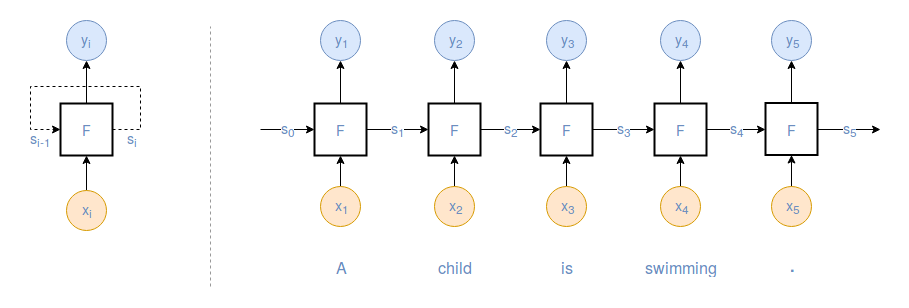
\includegraphics[totalheight=5.5cm]{fig/rnn.png}
	\caption{General architecture of a \ac{RNN} (left). Example sentence in an unrolled \ac{RNN} (right).}
	\label{fig:rnn}
\end{figure}
Maintaining an internal state $s \in \mathbb{R}^m$, for $m$-dimensional representations, the network recursively iterates over the input sequence $x$, aggregating in each timestep the previous state $s_{i-1} \in \mathbb{R}^m$ with the current input $x_i$ using the function $F$. This state is then used for the next iteration and output via a mapping function as $y_i \in \mathbb{R}^m$. Multiple implementation variants exist of $F$ and what is shared across iterations. \ac{LSTM}s for instance use several neural gates to learn what information should be used, output or forgotten. This procedure ca be seen with an example sentence yb unrolling the network in Figure \ref{fig:rnn} (right). In typial setups a neural network may either choose to use $s_t$ or $y_t$ for a sequence length of $t$ as the final sentence representation \citep{goldberg2017Apr}, since the network iterated over the full input sequence and contains the relevent information, if optimized for it. Even though the architecture of different versions of \ac{RNN} may be well understood and has a logical meaning, the actual procedure of deriving concrete representations within a trained model is hard to understand. We leverage the fact that the Shortcurt Stacked Encoder uses max-pooling over all $y_i$ to gather the sentence representation rather than using $y_t$ or $s_t$ by identifying what $y_t$ has the highest value within a given dimension and mapping this dimension to the word $x_t$ of the input sentence. As an example consider the sentence in Figure \ref{fig:rnn} (right). For each timestep $t$ a new vector $y_t$ is produced. As done by \cite{nie2017shortcut} we concatenate all $y_t$ to a matrix $\mathbb{R}^{m \times t}$, with $m$ being the representation size and each vector $y_t$ being the $t$th row within $M$. Assuming a dimensionality of $m = 3$, an examplatory matrix $M$ for the given sentence ``A child is swimming .'' is displayed in Figure \ref{fig:example_process_understanding}. 
\begin{figure}[tph!]
\centering
	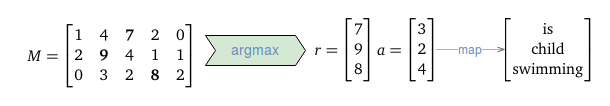
\includegraphics[totalheight=2cm]{fig/example_process_understanding.png}
	\caption{Visualized example of extracting interpretable information of the max-pooled seentence representations with a dimensionality of 3.}
	\label{fig:example_process_understanding}
\end{figure}
Additiobnally to creating the sentence representation $r$ by applying wor-wise max-pooling on $M$, we collect the vector $a$, containing the column indizes, that are responsible for the values within $r$. These can directly be mapped to the word of the source sentence and thus be interpreted by humans. It should be notted that due to the nature of the multi layer \ac{biLSTM} each $y_t$ does not only contain the word at $x_t$ but its context. While this somehow may lead to less accurate mapping, we found that the chosen method is sufficient to gain some meaningful insights on sentence encoding.

\paragraph*{Analysed data}
To reduce noise and aming for sentences that Shortcut-Stacked Encoder\textsuperscript{$\dagger$} seems to have a proper understanging about, we sample 1000 sentence representations from the \ac{SNLI} train data in the following strategy. We group all sentence pairs ($p$, $h$) sharing the same premise and only keep groups if all samples belonging to the same group are classified correctly. Thus, we reduce the amount of sentences that are definetly misunderstood by the model, that would be harder to interpret. For now we are not interested in the actual relation between $p$ and $h$ and therefore create a pool of the remaining sentences, by treating $p$ and $h$ equally and splitting their connections apart. After removing duplicate sentences, the most frequent sentence length for the remaining representations is 8. To reduce noise that may arise from different sentence lengths, we only consider sentences of a length of 8 and randomly sample 1000 sentence representations. All experiments in this chapter are based on the same instances, unless otherwise stated.
\newline

\noindent
In addition to the representation values each sample contains the following information:
\begin{itemize}
\item \textbf{Token:} The tokens that triggered the maximum value for the representation.
\item \textbf{Token position:} Positional information about the responsible tokens within the sentence.
\item \textbf{Lemma:} The lemmata of the responsible tokens.
\item \textbf{\ac{POS}:} The \ac{POS} tags of the responsible tokens.
\item \textbf{Dependency Parse:} The tags of the responsible tokens within the dependency parse tree.
\end{itemize}
Lemmatizing, \ac{POS}-Tagging and dependency parsing were conducted using spaCy.

\subsubsection{Detection of relevant dimensions}
manual research
identify relevant information
get understanding of the representation and how to interret it

create tool
label data and sort by label freqency + SD + dimension positions

responsible word i nitcht genug, value is immer wichtig
\subsubsection{Dimension-wise Analysis}
\paragraph{Positional information}
\paragraph{Semantic information}
\paragraph{Syntactic information}
\paragraph{Evaluation of the impact of female and male dimensions}
\subsubsection{Conclusion}
weg??
\subsection{Insights on the sentence alignment}\label{sec:insights_sent_alignment}
\subsubsection{Approach}
\subsubsection{Entailment analysis}
\subsubsection{Neutral and contradiction analysis}
\subsubsection{Experiments}
\subsubsection{Conclusion}
- eher experimental, need different models w maxpooling, mehr daten, mehr experiments, ...
\subsection{Errors of the base model}\newpage\cleardoublepage
\section{Additional SNLI test-set}\label{sec:additional_snli_set}
In the previous section we have identified several lexical inferences, that have not been captured by the model and thus mispredicted.  However we could only consider a small subset of misclassified samples, since a small lexical overlap would result in multiple interpretations of what the model understands and what not. In fact, even when identifying missing knowledge in our anaysis, we needed to rely on intuition rather than certainity when assigning mislabelled samples into categories. We also take a look about what the model seemingly knows, based on its correct predictions, shown in Table \ref{table:correct_samples}.
\begin{table}[!htbp]
\begin{center}
\begin{tabular}{lc}
\textbf{Premise/Hypothesis} & \textbf{Label} \\
\toprule
\specialcell{A young boy wearing a jacket pushing a hand mower on the grass.\\A girl is mowing the grass.} & \textit{contradiction} \\
\midrule
\specialcell{A man is doing a cannon ball into a pool, stadium chairs fill the background.\\Someone is jumping into water.} & \textit{entailment} \\
\midrule
\specialcell{A woman testing a comfortable pillow.\\The woman 's head is in contact with the pillow.} & \textit{entailment} \\
\bottomrule
\end{tabular}
\caption{Correctly classified examples.}
\label{table:correct_samples}
\end{center}
\end{table}
In the first example humans see, that both sentences describe the same scenario with only the main actor changing. Aiming for \ac{NLI} and thus \ac{NLU}, the model should proceed similarily. It cannot be said, whether the model identifies the paraphrasing of ``mowing''. Yet, we can see that the only required information for the correct label is the gender of the mowing person. This is, as we have seen in Section §\ref{sec:understanding}, a very important feature within the model. In the second sentence, an average human knows, that ``doing a cannon ball'' is a special form of ``jumping'' (in the water). However, a simple heuristic that $h$ is entailed by $p$ if it describes a more general scenario, would be sufficient for a correct prediction, if the model is able to identify that a ``man'' is a ``person'' and ``pool'' is somehow related to ``water''. Even the alignment to ``jumping'' and ``ball'' may be given in the representation, since the model mixed words in sportif/activity dimensions. Similarily, in the last sentence pair, we intuitively find it hard to believe, the process of ``putting the head in contact with the pillow'' is known to be implied when ``testing'' it to the model. Again, it seems more likely that the high overlap (and potentially the semantic relatedness of ``head'' and ``pillow'') are causing the correct prediction rather than actual \ac{NLU}. 

\subsection{Goal of the new test set}
We believe that the high accuracy on \ac{SNLI} stems from exploiting these simple heuristics, coming from dataset specifc patterns, rather than actually encoding the correct meaning of the sentences. Additionally, while models relying only on external information from distributed word representations achieve strong results, they still depend on the information encoded within these. Especially for mutually exclusive words, that appear in similar contexts, this information alone might not only be insufficient but also misleading. With this motivation, we create a new additional test set \citep{glockner_acl18} for \ac{SNLI} with adversarial sentence-pairs, that only differ in one aspect, defined by lexical semantic relations. This will help in three aspects:
\begin{itemize} 
\item We show that even state-of-the-art models fail to capture simple lexical inferences and a high performance on \ac{SNLI} is not sufficient evidence for a proper \ac{NLU}, being heavily dependant on dataset specific patterns. This is motivated by \cite{jia-liang:2017:EMNLP2017}, who find similar issues in the field of reading comprehension.
\item Having sentence-pairs, differing in only one specific and known aspect, enables a very accurate estimation, whether the model has enough understanding capabilites for the particular required lexical relation or not, as we exclude any noise.
\item Only measuring the capability for lexical inferences, that are available in a variety of lexical resources, like WordNet, we show the need to incorporate such knowledge bases into neural networks and provide a dataset, to measure the effectiveness of these approaches. Note that improvements (even if applied on the underlying \ac{NLU}) are hard to show on the original \ac{SNLI} test set, has models already achieve results at the upper possible bound.
\end{itemize}
Our claim, that state-of-the-art results highly overestimate the actual \ac{NLU} capabilities of the model, as they rely on patterns within the dataset, is in line with other works, that tackle the problem from different perspectives. \citep{gururangan2018annotation} refer to those patterns as ``Annotation Artifacts'', arising from similar stragies used by the annotators, when creating the hypothesis for each label. As opposed to our approach, they do not create new samples to reduce the impact of these patterns. Instead, they identify samples, that contain enough information solely in their hypothesis, to be classified correctly. After removing these samples, the remaining dataset shows, that state-of-the-art models perform significantly worse. \citep{dasgupta2018evaluating} focus on the compositional aspect by atomatically generating sentences from \ac{SNLI}, rearranging noun phrases in any order around the words ``\texttt{[not] more / less}'', thus requiring the model, to consider the sentence structure\footnote{For instance: ``The man has more hair than the woman.'' vs. ``The woman has more hair than the man.''}. Based on their results, they claim that the high performance on \ac{SNLI} arises from the fact, that word-overlaps or specific single word relations are often sufficient.

\subsection{Dataset}
We now describe, how we create the new test set and make sure it, that is correct and \textit{fair} w.r.t. the train data in the way, that it does not introduce new information, but only relies on the generalization ability of information, given in the train data. This is important, since we cannot assume a model trained on a specific dataset to perform equally good on different domains \citep{goldberg2017Apr}.
\subsubsection{Creation of adversarial samples}
We derive all new sentence pairs from the original \ac{SNLI} train set, by replacing selected expressions within a single sentence. Those expressions usually consist of a single word, however in some cases, like ``New Zealand'', it consists of several words, according to our definition. For the sake of simplicity, in the remainder of this chapter, we generally speak of \textit{words} rather than \textit{expressions}, covering all of our replacements. The original sentence from \ac{SNLI} is kept as the premise, while the adapted sentence with the replaced word, serves as the hypothesis. We will in the remainder of thes section refer to $w_p$ for the word within $p$ that was replaced by the word $w_h$ in $h$. Samples from the resulting dataset are shown in Table \ref{tab:new_testset_samples}.
\begin{table}[htt]
\centering
\begin{tabular}{lc}
\toprule
	\textbf{Premise/Hypothesis} & \textbf{Label} \\  \midrule
		The man is holding a saxophone & \multirow{2}{*}{contradiction} \\
        The man is holding an electric guitar & \\
        \midrule
		A little girl is very sad. & \multirow{2}{*}{entailment} \\ 
        A little girl is very unhappy.&  \\
        \midrule
		A couple drinking wine & \multirow{2}{*}{neutral} \\
        A couple drinking champagne &  \\
    \bottomrule
  \end{tabular}
  \caption{Examples from the newly generated test set.}
    \label{tab:new_testset_samples}
\end{table}
Note that traditional \ac{RTE} systems would consider the first example as neutral, since a man may hold both instruments at the same time. However for being conform with the labelling scheme in \ac{SNLI}, this is considered as contradicting\footnote{We verified this by finding similar samples within the actual \ac{SNLI} dataset, also labelled as contradiction.}, based on the event-coreference assumption and the most dominant aspects of the image being  described within the sentence. This was introduced by \cite{bowman2015large} for exactly this purpose of distinguishing between different interpretations and hence reducing ambiguity of different possible labels.

\paragraph*{Generation of word-pairs}
We manually generate a list of word-pairs ($w_p$, $w_h$) from online resources for English Learning \footnote{\href{http://www.enchantedlearning.com}{http://www.enchantedlearning.com}}. They provide large lists topically clustered words, which we use to derive co-hyponyms, as well collections of as rather generally applicable synonyms or antonyms. We focus partly on entailing, but mostly on contradicing examples, and assume synonyms to refer to the former, co-hyponyms and antonyms to the latter case. Doing so we must consider the following things:
\begin{itemize}
\item \textbf{Compatible co-hyponyms:} Co-hyponyms not necessarily exclude each other \citep{kruszewski2015so}. A ``jongleur'' for instance might also be a ``clown'', even though both could be considered as neighbouring hyponyms of artist, while a ``horse'' and a ``cow'', both hyponyms of ``animal'' may not both refer to the same entity. As the newly generated sentence-pairs naturally will have a high lexical overlap, the prediction may be emphasized towards neutral anyway because if some distinct information. To reduce the impact of this rather random decison criteria, we mostly aim to find out, whether the model is able to identify contradicting examples. Thus, we focus on mutually exclusive rather than compatibe co-hyponyms. Similarily, we remove word-pairs, that commonly are confused by humans like ``pink'' vs. ``purple''. 
\item \textbf{Polysemy:} In order to automatically generate new sentences from ($w_p$,$w_h$), we require both words to have one highly dominant sense, such that both words are generally replacable, leading to correct sentences. We verify this, by sampling random sentences, containing $w_p$, to see their usage within \ac{SNLI} is conform with $w_h$. Words that appear in highly different senses are excluded. The country ``Jordan'' for instance, is mostly used in the sense of the basketball player \textit{Michael Jordan}, and thus is not used. We observe a similar problem on much more fine-grained level. The word-pair of the antonyms (\textit{old}, \textit{young}) both contradict each other on a very general basis. Yet, whether they can be replaced or not is dependant on the context. While ``old'' may refer to \textit{things} as well as people (like ``an old computer'' or ``an old man''), ``young'' usually can only be used in combination with people. We thus distinguish between ($w_p \leftrightarrow w_h$), that can be swapped both ways, and ($w_p \leftarrow w_h$), that only can be swapped in one direction. In this case the more restricted term ``young'' can be replaced by ``old'', not vice versa, as we aim for a high precision on correct sentences.
\item \textbf{Structural word usage:} Furthermore, ($w_p$, $w_h$) may be used together with different function words. Consider the for instance (``day'', ``night'') or (``near'', ``far''). While both ($w_p$, $w_h$) represent opposite meanings for a high amount of contexts, replacing one with each other leads to invalid sentences like ``John sleeps at day[/night]'' or ``The house is very near[/far] from the sea''. We identify these patterns by looking at the word usage, and extend the ($w_p$,$w_h$) adequatly with the function words like (``during the day'', ``at night''), automatically reducing the chance of incompatible senses as a side-effect.
\end{itemize}
We manually evaluate all selected ($w_p$,$w_h$) for synonyms and antonyms, based on the points mentioned above. Topic related co-hyponyms are only individually evaluated, as mapping each word with each of its co-hyponyms is rather inefficent to manually verify. In addition to that, we create antonym word-pairs from WordNet, sharing the same \ac{POS} and having a cosine similarity of $\geq 0.5$. In total we generate 3990 word-pairs\footnote{We count the replacement directions separately, thus ($w_p \leftrightarrow w_h$) counts as ($w_p \rightarrow w_h$) and ($w_p \leftarrow w_h$).} and keep the topical (in case of cohyponyms) or relational (for synonyms and antonyms) information, leading to 13 groups\footnote{Countries, Nationalities, Colors, Numbers, Antonyms, Synonyms, Vegetables, Drinks, Loction-Verbs, Materials, Planets, Rooms, Instruments}. To ensure that we not confront the models, trained on \ac{SNLI}, with new information, we verify that each word indeed is within the train-data and the used word-embeddings. In the final test set, frequencies\footnote{The amount of individual sentences containing $w_h$ in the exact surface form.} from newly introduced words $w_h$ range from a single occurence (e.g. ``Portugal'') up to 248,051 occurences (``man'') with a mean of 3,663.1 and a median of 149.5 (interquartile range 19.0 - 1107.5). As the general goal of machine learning is not to memorize, we aim for this distribution, having a high amount of less representative words, to measure the models generalization power. We motivate this, as it is very likely in a real-world scenario, to encounter samples requiring this kind of knowledge, even though it may not be omnipresent within the train data, and hence should be inferred from the learned features.

\paragraph*{Generation of sentence-pairs}
As previously mentioned, we derive all our samples from premises of from the training set. Theses premises serve in the exact same form as the premise of our new samples, while the hypothesis is generated by replacing $w_p$ within $p$ by $w_h$. Thus, not only are the newly introduced words known from the training process, but also each $p$ has been seen during training in the exact same form, and has been encoded with respect to at least three hypothesis, for each label respectively\footnote{Due to the generation process of \ac{SNLI}.}. By doing so, we intentionally violate common practives in machine learning, as the test set is not completely isolated from the train data, wich should serve as an advantage for the model. We finally remove highly unlikely sentences by ensuring that the bigrams  ($w^{t-1}$,$w_h^t$) and ($w_h^t$, $w^{t+1}$) with $w^t$ being the $t$th word within $h$ must have a frequency of at least 10 in the wikipedia bigram corpus\footnote{\href{https://github.com/rmaestre/Wikipedia-Bigram-Open-Datasets}{https://github.com/rmaestre/Wikipedia-Bigram-Open-Datasets}}. In case the replacement consists of several words, $w^t_h$ corresponds to the first or last word of this expression respectively. This preprocessing helps to clean the created samples, yet two problems remain.

\paragraph*{Remaining issues}

Especially on the semantic level, our newly created sentences may still be incorrect. For instance consider the following sentence-pair:
\begin{center}
\begin{tabular}{rl}
\textbf{Premise:} & The car would not \textit{start} and, consequently, stayed in this garage. \\
\textbf{Hypothesis:} & The car would not \textit{end} and, consequently, stayed in this garage.
\end{tabular}
\end{center}
Obviously both bigrams (``not'', ``end'') and (``end'', ``and'') appear quite commonly within a large text corpus. However does ``end'' neither serve as an appropriate verb for ``car'', nor would the resulting sentence (even if a more applicable word like ``stop'' would be used) make any sense to a human.
\newline

\noindent
Furthermore, we need to assign the correct label for the relationship between both sentences. Knowing that our newly created $p$ and $h$ only differ in one word, one could consequently assume that the relationship between $p$ and $h$ is the same the relation between $w_p$ and $w_h$. Thus for instance, one could label ($p$,$h$) as contradiction, if $w_p$ and $w_h$ exclude each other, or as entailment, if they have synonym meanings. This heuristic may indeed be correct for most cases. \cite{maccartney2007natural} however show, that this is only the case for upward-monotone sentences. In upward-monotone sentences, replacing a word (e.g. ``cow'') with a more general term, like a hypernym (e.g. ``animal''), yields in a broader meaning coverage of the sentence and thus results in entailment. \cite{maccartney2007natural} identify several linguistic patterns, like negation or restrictive quantifiers (e.g. ``without'') or verbs (e.g. ``fail''), that result in downward-monotone sentences, yielding to different results w.r.t. entailment relation. This differentiation is not only relevant for hypernyms but also for other lexical relations, as shown in Table \ref{tab:monoton_samples} with the example of co-hyponyms.
\begin{table}[htt]
\centering
\begin{tabular}{c|lc}
& \textbf{Sentences} & \textbf{Label} \\
\toprule
\specialcellc{\textbf{Upward}\\\textbf{monotone}} & \specialcell{John is hiking in \textit{France}\\John is hiking in \textit{Italy}} & contradiction \\
\midrule
\specialcellc{\textbf{Downward}\\\textbf{monotone}} & \specialcell{John is hiking outside of \textit{France}\\John is hiking outside of \textit{Italy}} & neutral \\
\bottomrule
\end{tabular}
 \caption{Comparison of co-hyponyms in upward-monotone and downward-monone sentences.}
 \label{tab:monoton_samples}

\end{table}
In both examples ``France'' is replaced by its co-hyponym ``Italy''. Even though both words are mutually exclusive only for the upward-monotone sample, the sentence relation reflects the relation between both words. The same implication does not hold anymore for the downward-monotone sentence. Even though we can assume that most premises in \ac{SNLI} are upward monotone, especially since image captionas are more likely to explicitly describe the content of the picture, we must take into account, that whether the sentence relations corresponds to the relation of ($w_p$,$w_h$) or not, depends on the context of these words.

\subsubsection{Validation}
We address both mentioned problems, by annotating the new test set using crowd-sourcing with Amazon Mechanical Turk\footnote{\href{https://www.mturk.com/}{https://www.mturk.com/}}. In order to make this a cost-effective process, we aim for the \ac{HIT} to be simple for the annotators while at the same time enabling them, to validate and label as many as possible samples. We constrain ourselves, such that one \ac{HIT} contains five hypothesis, which are all originating from the same premise. This way annotators must only read the premise once, to compare it with those newly created sentences. Not all our identiffied categories of word-pairs are well represented. In order to get the most of our less frequent categories, we sample the 10,000 sentence-pairs, that need to be annotated, in a greedy manner: After soring categories by the amount of samples, that we created, we start with the least representative categories and sample as many sentence-pairs as possible, keeping our constraint of needing a multiple of five hypothesis per premise up to an upper bound of samples per category\footnote{The upper bound is always re-calculated, serving the purpose of not sampling too much of one category, since the amount of all samples is bound at 10,000.}. If more samples are required to complete a \ac{HIT} with five hypothesis, the next categories are checked in the order of representativeness. Furthermore we keep track of the amount of each word-pair, that is included in the sampled sentence-pairs, and always prefer less-frequent word-pairs, if several options exist.
\paragraph*{Annotation process}
To simplify the \ac{HIT}s for annotators, such that they do not need to understand the labelling scheme of \ac{SNLI}, we create a set of questions, highly aligned\footnote{\cite{bowman2015large} only provide their annotation guidelines for the task of creating new hypothesis, not for validating them. The validation task was conducted separately and was only open for annotators who participated in the hypothesis-generation task and thus were qualified already. } with those, proposed of \cite{bowman2015large}, that we later map to entailment labels. Specifically, we ask:
\begin{enumerate}
\item if both sentences describe \textbf{the same event}
\item if the hypothesis \textbf{adds new information}
\item if the sentence is \textbf{invalid}
\end{enumerate}
Samples that are answered negatively for (1) result in the label \textit{contradiction}. If (1) is answered positively, the label is either \textit{neutral}, if (2) is answered positively, or \textit{entailment}, if (2) is answered negatively. Sentences that show major grammatical errors or do not make sense to a native English speaker, should be marked using (3) and no label is inferred. We defined the \ac{HIT} user interface such that no other combinations can be selected as an answer. The questions are explained in deeper detail in an additional introdcution, and we ensure they are understood correctly with a mandatory qualification test. Since \ac{SNLI} does contain grammatical and spelling errors, we specifically allowed minor errors of that kind. Additionally, \ac{SNLI} does contain fictive sentences that are not realistic. Yet, it is hard to define the degree that sentences are allowed to sound unrealistic. While ``flying to school'' instead of ``walking to school'' may a bit unrealistic but still plausible for a fictive scenario, ``sitting at the table and eating'' and ``walking at the table and eating'' seems indeed very unlikely. This however, is highly dependant on the subjective perspective. We defined this aspect of (3) rather swammy, by allowing fictive scenarios, however counting on the English capabilities of native speakers, to identify if those sentences make sense to them and seem like a proper usage of words. Due to this loose definition, we strictly ignore all samples, if at least one single annotator marked them as invalid, not requireing a majority in this case. To assure, that our workers have shown to annotate appropriately to the task description, we only accept annotators with an approval rate of at least 99\% and a minimum of 1,000 prior tasks. A sample \ac{HIT} is shown in Figure \ref{fig:example_hit}. 
\begin{figure}[tph!]
\centering
	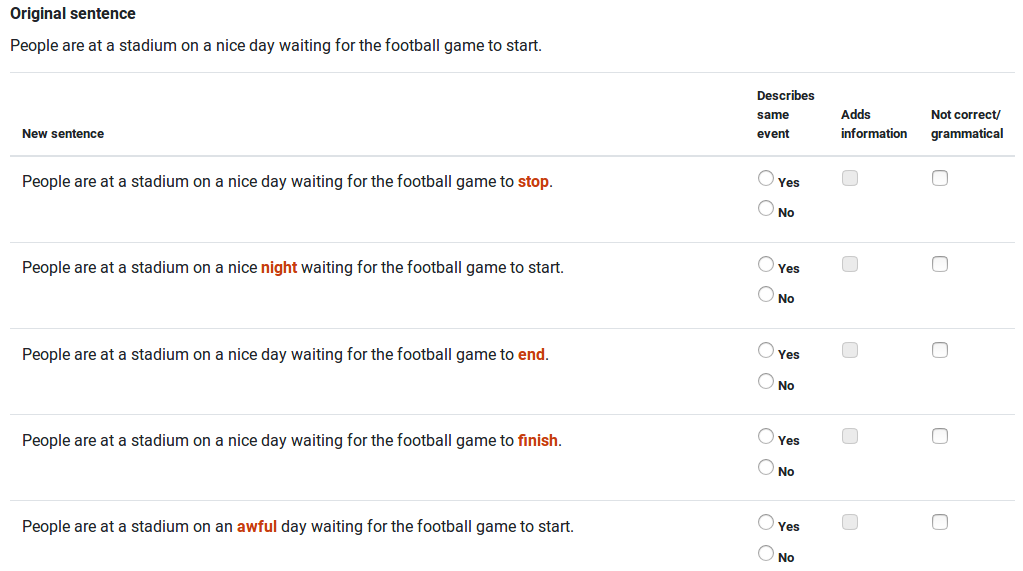
\includegraphics[totalheight=7cm]{fig/sample_hit.png}
	\caption{Example of a \ac{HIT} in Amazon Mechanical Turk.}
	\label{fig:example_hit}
\end{figure}
The questions are explained to the users with example \ac{HIT}s of the same form in the instructions. In order to make the task more attractive to annotators, without increasing the payment too much, we simplified the process by highlighting the exchanged words.
\newline

\noindent
We assign each \ac{HIT} to three annotators. After removing all invalid sentence-pairs, we consider the majority label as the gold label, if at least two annotators agree on it. Sentence-pairs without agreement are not considered for our new testset. After an inital annotation round of 1,000 samples, we remove categories and word-pairs, that show a high tendency of having invalid sentences. We show the statistics of our final testset, consisting of 8,193 sentence-pairs in Table \ref{tab:newtest_stats}.
\begin{table}[tph!]
\centering
\begin{tabular}{l|cccc|ccc}
& \multicolumn{4}{c}{\textbf{Instances}} & \multicolumn{3}{c}{\textbf{Fleiss $\kappa$}} \\
& contradiction & neutral & entailment & \textbf{Overall} & contradiction & entailment & \textbf{Overall} \\
\toprule
\textbf{SNLI Test}& 3,236 & 3,215 & 3,364 & \textbf{9,815} & 0.77 & 0.69 & \textbf{0.67} \\
\textbf{New Test}& 7,164 & 47 & 982 & \textbf{8,193} & 0.61 & 0.90 & \textbf{0.61} \\
\bottomrule
\end{tabular}
	\caption{Statistics of \ac{SNLI} testset compared with the newly generated testset.}
	\label{tab:newtest_stats}
\end{table}
As can be seen, the new test set is heavily focused on contradicting samples. Since this test set only serves, to measure the capabilities of a model in dealing with lexical inferences (and \ac{NLU} with reduced dataset-specific patterns), but not to replace the original \ac{SNLI} testset, this is not problematic. It still must be considered, when evaluating a model, as a simple baseline, predicting everything as contradiction, would result in an accuracy of 87.4\%. We report the agreement with Fleiss Kappa \citep{landis1977measurement} (over all samples and for the representative labels \textit{entailment} and \textit{contradiction}), as it was done by \cite{bowman2015large} for the original \ac{SNLI}. For better comparison, we re-calculate the numbers on all valid samples of the \ac{SNLI} testset. The new testset yields ``substantial agreement'' with a Fleiss Kappa of 0.61. It should be noted, that Kappa also considers, how likely a specific label would selected by chance, and for this purpose takes the overall label distribution into account. This does not influence the measure for the original \ac{SNLI}, since all labels are evenly distributed. For the new test set however, this method assumes that contradiction is more likely to appear by chance, due to its high frequency. As this results from our selected word-pairs rather than an underlying ``natural distribution'', the figure, calculated by Fleiss Kappa, might be less suited as an agreement measure for the new dataset. Yet, for very different reasons, it is indeed likely that annotators are slightly biased towards selecting contradiction, as the result of our \ac{HIT} presentation: Since most word-pairs are contradicting and word differences are highlighted, annotators might, to some extend, shift their focus more on the difference between those words, rather than solely on the actual word-usage in context. To provide an easier to interpret measure of this dataset, we estimate the human performance in the same manner, as done by \cite{gong2017natural} for \ac{SNLI}. They consider all samples with majoriy label, which results in the gold label, and calculate the ratio of annotator labels, matching the majority gold label, as the estimate for the human performance in terms of accuracy. Thus, let $g(x,y)$, with $x$ as the annotator label and $y$ as the estimated gold label, define, if the annotation counts as a misclassification or not:
\begin{equation}
g(x,y) = \begin{cases}
1 & \text{if $x = y$} \\
0 & \text{if $x \neq y$ }
\end{cases}
\end{equation}
Let furthermore $L$ contain all pairs $(x,y)$ of the annotated dataset and $|L|$ be the amount of elements within $L$. Following \cite{gong2017natural}, we estimate the human performance $a$ in accuracy as follows:
\begin{equation}
a = \frac{\sum_{(x,y) \in L} g(x,y)}{|L|}
\end{equation}
Doing so, we estimate the human performance on the new testset to be 94.1\%, slightly higher than the human performance estimated on \ac{SNLI} with only 87.7\%, indicating that our new sentence-pairs do not pose additional difficulties, but in fact indeed seem relatively easy for humans.
\subsection{Evaluation}
We evaluate three neural models without external knowledge other than the one from distributed word-embeddings, that achieve strong results on \ac{SNLI}. All models are retrained with different datasets, using the provided code and keeping all hyperparameters. We explain the experimental setup and results below. 
\subsubsection{Experimental setup}
\paragraph*{Models without external knowledge}
We evaluate the Residual-Stacked Encoder\textsuperscript{$\Diamond$} \citep{nie2017shortcut}, as explained in Section §\ref{sec:residual_encoder_def}, ESIM \citep{chen2017enhanced} and Decomposable Attention \citep{parikh2016decomposable}, both explained in Section §\ref{sec:models_snli}. The published model of ESIM ensembles two models with different sentence encoding strategies, one is based on a TreeLSTM, the other on a \ac{biLSTM}. For our experiments we retrain only the \ac{biLSTM}-based model. For Decomposable-Attention, we use the AllenNLP re-implementation\footnote{\href{http://allennlp.org/models}{http://allennlp.org/models}}. As opposed to the reported version on the SNLI leaderboard\footnote{\href{https://nlp.stanford.edu/projects/snli/}{https://nlp.stanford.edu/projects/snli/}} this implementation does not use the optional intra-sentence attention. Its performance on the \ac{SNLI} test is with 84.7\% slightly lower, but comparable to the model with intra-sentence attention (86.3\%). All models have different characteristics, depticted in Table \ref{tab:compare_architecture_models} and are at the time of the experiment amongst the best within their categories.
\begin{table}[tph!]
\centering
\begin{tabular}{r|ccc}
& \specialcellc{\textbf{Finetune}\\\textbf{Embeddings}} & \textbf{LSTM-based} & \specialcellc{\textbf{Inter-sentence}\\\textbf{Attention}} \\
\toprule
Decomposable Attention \citep{parikh2016decomposable} & $-$ & $-$ & \textit{yes}\\
Residual-Stacked Encoder \cite{nie2017shortcut} &\textit{yes}  &\textit{yes} & $-$\\
ESIM \citep{chen2017enhanced} &\textit{yes} &\textit{yes} & \textit{yes}\\
\bottomrule
\end{tabular}
\caption{Architectural comparison of tested neural models without external knowledge.}
\label{tab:compare_architecture_models}
\end{table}

\subsubsection{Models with external knowledge}
Additionally we also provide a simple WordNet baseline, predicting the relationship of ($p$,$h$) by assuming all sentences to be upward-monotone and, thus having the same relation as ($w_p$,$w_h$). Specifically, for each ($w_p$,$w_h$) we check their lexical semantic relation within WordNet, and map it to a relation label in the following manner:
\begin{itemize}
\item \textbf{Synonymy:} Synonyms are predicted as \textit{entailment}.
\item \textbf{Antonomy:} Antonyms are predicted as \textit{contradiction}.
\item \textbf{Hypernomy:} If $w_p$ is a hypernym of $w_h$ the sentence-pair is predicted as \textit{neutral}, if $w_p$ is a hyponym of $w_h$ as \textit{entailment}.
\item \textbf{Co-hyponomy:} Cohyponyms are predicted as \textit{contradiction}. We only only consider co-hyponyms with a maximum distance of two edges in the ontology to their common hypernym, as considering all potential co-hyponyms would yield all ($w_p$,$w_h$) coming from the same (very general) root-word to be labelled as contradiction.
\end{itemize}
We map multi-word expressions like ``at night'' to their meaning-carrying word (``night''), if the function words have only been added for a higher precision, when replacing the words in the generation process. In case they refer to actual entities (e.g. ``New Zealand''), we identify the applicable synsets of the whole expression in WordNet. As explained in Section §\ref{sec:wordnet}, words may have several synsets leading to potentially several different lexical relations amongst the words of interest $w_p$ and $w_h$. For each relation between both words, we calculate a score $s=\max(r_p,r_h)$ with $r_p$ and $r_h$ being the rank of the synset of the word $w_p$ and $w_h$ respectively. This follows the common heuristic that dominant senses appear as the first synsets while rare senses appear at the end \citep{mccarthy2004using}. Subsequently, if several lexical relations exist, we consider the one with the lowest assigned score as tie-breaker\footnote{In case the score $s$ is identical for several relations, we select the relation in the following order ($X > Y$ meaning $X$ is preferred over $Y$):\\ synonym $>$ antonym $>$ hypernym $>$ hyponym $>$ co-hyponym } and thus, tend to focus on more dominant word-senses. Of course, this baseline only is possible, if knowing that $p$ and $h$ only differ in $w_p$ and $w_h$ and is thus not applicable to sentence-pairs in general. Yet it provides insight, to what extend information within WordNet can help on our new test set. In addition to that we, also report\footnote{We did not conduct the experiment with \ac{KIM} ourselves, but received their results from the orignal authors recently. The analysis part thus does not contain deeper analysis of the performance of KIM.} the results of \ac{KIM} \citep{chen2017natural}, as explained in Section §\ref{sec:rel_work_sentence_encoding_models}.
\paragraph*{Traing data}
In addtion to training all models on \ac{SNLI}, wich is considered relatively easy, we also train each model on the union of SNLI and \ac{MultiNLI} and SciTail respectively, both are assumed to be more difficult and explained in deeper detail in Section §\ref{sec:basics_datasets}. The motivation is, that while SNLI might lack the training data needed, to learn the required lexical knowledge, this data may be available in the other datasets, which are presumably less simple. 
\subsubsection{Results}
The results for each model with the according train sets are visualized in Table \ref{tab:adv_results}.
\begin{table}[tph!]
\centering
\begin{tabular}{c c c c c c}
\toprule
\textbf{Model} & \textbf{Train set} & \textbf{SNLI test set} & \textbf{New test set} & $\Delta$ \\ 
\midrule
\multirow{3}{*}{\specialcellc{Decomposable Attention \\ \citep{parikh2016decomposable}}} & SNLI & 84.7\% & 51.9\% & -32.8 \\ 
& MultiNLI + SNLI & 84.9\% & 65.8\% & -19.1 \\ 
& SciTail + SNLI & 85.0\% & 49.0\% & -36.0 \\ 
\midrule
\multirow{3}{*}{\specialcellc{ESIM \\ \citep{chen2017enhanced}}} & SNLI & 87.9\% & 65.6\%& -22.3\\ 
& MultiNLI + SNLI & 86.3\% &74.9\% & -11.4\\
& SciTail + SNLI & 88.3\% & 67.7\%& -20.6\\ 
\midrule
\multirow{3}{*}{\specialcellc{Residual-Stacked Encoder\textsuperscript{$\Diamond$} \\ \citep{nie2017shortcut}}} & SNLI & 86.0\% & 62.2\% & -23.8\\ 
& MultiNLI + SNLI & 84.6\% & 68.2\%& -16.8\\ 
& SciTail + SNLI & 85.0\% & 60.1\%& -24.9\\ 
\midrule
WordNet Baseline & - & - & 85.8\% & - \\ 
KIM \citep{chen2017natural} & SNLI & 88.6\% & 83.5\% & -5.1 \\ 
\bottomrule
\end{tabular}
\caption{Results of models on the new test set compared with the original \ac{SNLI} test set.}
\label{tab:adv_results}
\end{table}
There is a clear trend, that adding \ac{MultiNLI} to the training data boosts the model's performance on the new test set. At the same time it decreases the test accuracy on SNLI, indicating that the performance, gained on \ac{SNLI} test, does not reflect the true \ac{NLU} capabilities, since clearly less lexical semantic relations are understood. Yet, compared with the original estimated performance, even by almost doubling the amount of train data with \ac{MultiNLI}, all models without external knowledge show a significant drop in performance. While MultiNLI follows the same labelling scheme as SNLI, and thus is compatible, SciTail does not specifically assume event coeference and lacks having the label \textit{contradiction}, which is dominant in the new test set. Hence, the models seem to not be able to leverage from the extended amount of data in this case. Both models with WordNet information perform significantly better than the ones without. This shows, that the lexical relations, as contained in WordNet, are sufficient to gain strong improvements on the new dataset. In addition to that, those relations have also shown to be useful for \ac{KIM} in training on \ac{SNLI} (as they are considered for the prediction). This especially shows some crucial drawbacks in the neural models without WordNet, as they clearly lack to extract those features when trained solely with textual input, by learning features based on arbitrary patterns at the cost of also meaningful (for \ac{SNLI} and naturally for \ac{NLU}) features of lexical relations. Only dropping by 5.1 points in accuracy w.r.t. the performance on \ac{SNLI}, \ac{KIM} seems substentially more stable, when sentences are adapted, forcing the model to predict based on a language understanding rather than dataset specific patterns. This of course may be due to the fact, that the new testset, being closely related to the train data and requiring the same knowledge, as added for \ac{KIM}, is highly suitable for\ac{KIM}. Thus, it still does not prove truely superior \ac{NLU}, yet it shows that they found a successful strategy of integrating this resource into neural models.

\subsection{Analysis}
We take a closer look on the performance achieved by the models without external knowledge. As the performance only improves marginally, if the train data is tremendously increased by adding \ac{MultiNLI}, we focus our analysis part on the models, solely trained on the original \ac{SNLI} dataset.
\subsubsection{Accuracy by category}
Table \ref{tab:acc_by_cat} shows the accuracy per category, as defined when creating the word-pairs, for all models, including \ac{KIM} and the WordNet baseline. As not all categories contain an even amont of sanples, we additionally supply information about this figure, together with sample words for a better understanding, what each category represents. Originating from our word-pairs, almost all categories are majority labelled contradiction, solely synonyms mostly are labelled as entailment.
\begin{table}[tph!]
\centering
\begin{tabular}{lrc|ccccc} 
\toprule
\textbf{Category} & \textbf{Amount} & \specialcellc{\textbf{Example}\\\textbf{Words}} & \specialcellc{\textbf{Decomposable}\\\textbf{Attention}} & \textbf{ESIM} & \specialcellc{\textbf{Residual}\\\textbf{Encoders}} & \specialcellc{\textbf{WordNet}\\\textbf{Baseline}} & \textbf{KIM}  \\ \midrule
antonyms & 1,147 & \textit{loves - dislikes} & 41.6\% & 70.4\%& 58.2\% &  95.5\% & 86.5\% \\ 
cardinals & 759 &\textit{five - seven} & 53.5\% &75.5\% & 53.1\% & 98.6\% & 93.4\% \\ 
nationalities & 755 & \textit{Greek - Italian} & 37.5\% &35.9\% & 70.9\% & 78.5\% & 73.5\% \\ 
drinks & 731 & \textit{lemonade - beer} & 52.9\% &63.7\% & 52.0\% & 94.8\% & 96.6\% \\ 
antonyms (WN) & 706 & \textit{sitting - standing} & 55.1\% & 74.6\%& 67.9\% & 94.5\% & 78.8\% \\
colors & 699 & \textit{red - blue} & 85.0\% &96.1\% & 87.0\% & 98.7\% & 98.3\% \\ 
ordinals & 663 & \textit{fifth - 16th} & 2.1\% &21.0\% & 5.4\% &40.7\% & 56.6\% \\ 
countries & 613 & \textit{Mexico - Peru} & 15.2\% &25.4\% & 66.2\% & 100.0\% & 70.8\% \\ 
rooms & 595 & \textit{kitchen - bathroom} & 59.2\% &69.4\% & 63.4\% & 89.9\% & 77.6\% \\ 
materials & 397 & \textit{stone - glass} & 65.2\% & 89.7\%& 79.9\% & 75.3\% & 98.7\% \\
vegetables & 109 & \textit{tomato -potato} & 43.1\% &31.2\% & 37.6\% & 86.2\% & 79.8\% \\ 
instruments & 65 & \textit{harmonica - harp} & 96.9\% &90.8\% & 96.9\% & 67.7\% & 96.9\% \\ 
planets & 60 & \textit{Mars - Venus} & 31.7\% & 3.3\%& 21.7\% & 100.0\% & 5.0\% \\ 
\midrule
synonyms & 894 & \textit{happy - joyful} & 97.5\% & 99.7\% & 86.1\% & 70.5\% & 92.1\% \\ 
\midrule
total & 8,193 &  & 51.9\% &65.6\% & 62.2\% & 85.8\% & 83.5\% \\ 
\bottomrule
\end{tabular}
\caption{Accuracy reached for the tested models for each category with assoziated sample words and the amount of instances.}
\label{tab:acc_by_cat}
\end{table}
All neural models achieve good results on categories that occur very frequently within \ac{SNLI} in general, like \textit{colors}. Also \textit{instruments} are well captures. We find that muscic instruments often occur in SNLI in very similar sentences containing some kind of \texttt{actor} and in conjunction with the instrument and the verbs "hold" or especially "play". In contradicting samples of the train data, in most cases the instrument changes. Thus our newly created sentence-pairs are very similar to those within the train data, explaining the good performance within that category. On the other hand, categories that are rare in \ac{SNLI}, like \textit{planets} or \textit{ordinals}, are not well understood by those models. As opposed to to \textit{instruments}, the relevance of \textit{ordinals} within a sentence in \ac{SNLI} usually is less crucial. Yet this originates only the commonly applied strategies by the annotators, as identified by \cite{gururangan2018annotation}. Consider for instance the sentence ``"A man racing his motorcycle comes in \textit{first}."'', which naturally yields in contradiction if we replace ``first'' by ``eights''. Yet the model without external information seemingly do not differentitate between both ordinal numbers, as annotators rather tend to change ``man'' or even ``motorcycle'', but not ``first''. Also \textit{drinks}, \textit{vegetables} and \textit{rooms} are generally harder for the model to predict for similar reasons. The reason for \textit{antonyms} being more difficult  than \textit{antonyms\_WordNet} most like arises from the fact, that they include gender-related antonyms, appearing in SNLI in abundance, that we do not include within the hand-crafted word pairs. As \textit{synonym} examples have large lexical overlap and differ only by one word, occuring in similar contexts (and subsequentially having a similar word-vector), it is no surprise, that all models achieve a good performance here. Inter-sentence-attention seems to have an advantage in this case, since only the Residual-Stacked Encoders does not improve significantly over its original test performance. We thus focus the remaining part of the analysis on contradicting sentence-pairs only.

\subsubsection{Impact on the word embeddings}
As previously pointed out, word-pairs with the lexical semantic relations, antonymy and co-hyponynomy, in many cases result in similar word representations with distributed embeddings. Subsequentially, we first analyse the impact of those word-representations, leveraging from the fact, that sentence-pairs in our new dataset only differs in one known word.
\paragraph*{Without fine-tuned embeddings}
Figure \ref{fig:decomp_acc_per_cos_sim} visualizes the performance of all contradicing samples, compared to the cosine similarity between the word-vectors of $w_p$ and $w_h$, achieved by Decomposable Attention. 
\begin{figure}[tph!]
\centering
	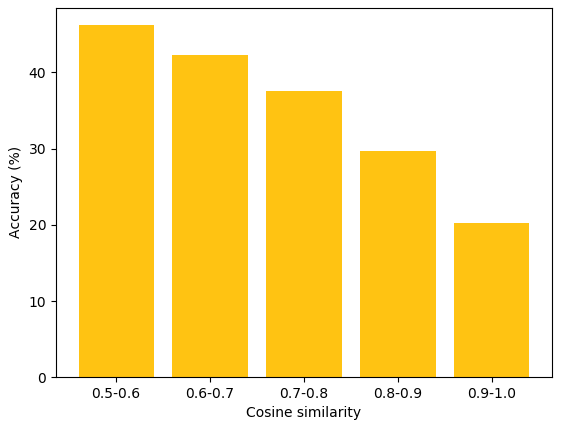
\includegraphics[totalheight=5cm]{fig/acc_by_cos.png}
	\caption{Accuracy by cosine similarity reached by Decomposable Attention (without fine-tuned embeddings).}
	\label{fig:decomp_acc_per_cos_sim}
\end{figure}
We exclude any multi-word expressions in this analysis. Let $v_p$ and $v_h$ be the word vectors of the GloVe embeddings, used by Decomposable Attention, the according cosine simmilarity $\cos(v_p,v_h)$ is calculated as follows:
\begin{equation}
\cos(v_p,v_h) = \frac{v_p v_h}{|v_p| |v_h|}
\end{equation}
We observe, that without fine-tuned embeddings, the reached accuracy highly correlates with the similarity of the word representations even though Decomposable Attention uses only the lower-cased word embeddings and thus contains comparably more samples per word-vector than the other two models, ESIM and Residual-Stacked Encoder. Those models rely on cased word-embeddings, and we could not find the same correlation between the accuracy and word-similarity. We assume this stems from the fact, that both models fine-tune embeddings and thus push contradicting words, as seen in the training, further apart in the embedding space. 
\paragraph*{With fine-tuned embeddings}
We evaluate the accuracy of both models with fine-tuned embeddings w.r.t. the amount $w_p$ and $w_h$ seen during training on \ac{SNLI} and visualize the results in Figure \ref{fig:esim_res_acc_by_freq}.
\begin{figure}[tph!]
\centering
	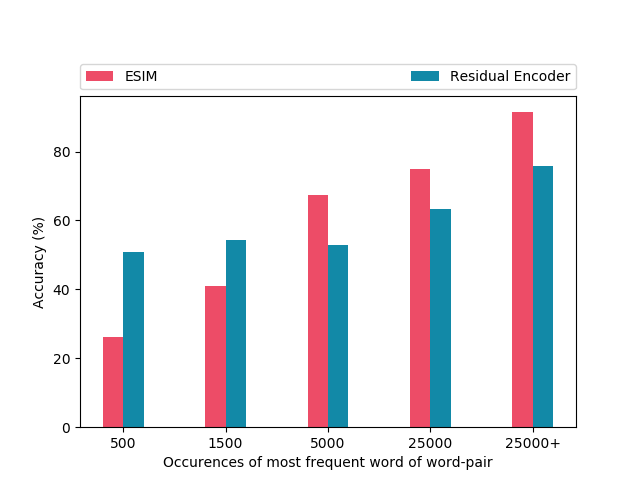
\includegraphics[totalheight=6cm]{fig/esim_res_acc_by_freq.png}
	\caption{Accuracy by word freqency for Residual-Stacked Encoder and ESIM.}
	\label{fig:esim_res_acc_by_freq}
\end{figure}
The numbers on the x-axis show the upper bound of word occurences of the word-pair, denoted as $a_{(w_p,w_h)}$, responsible for creating each sentence-pair. Specifically, we calculate the $a_{(w_p,w_h)}$ by taking the more frequent word within \ac{SNLI} train data, thus $a_{(w_p,w_h)} = \max(a_{w_p},a_{w_h})$, with $a_{w_p}$ and $a_{w_h}$ being the amount of sentences, containing $w_p$ and $w_h$ respectively. In case, one of $w_p$ or $w_h$ is an expression containing multiple words, denoted as $e = [w_1, \ldots , w_{n-1}, w_{n}]$, we calculate the according amount, denoted as $a_e$, by considering the least frequent word: $a_e = \min(w_1, \ldots , w_{n-1}, w_n)$. Intuitively, this will ignore added function words and, in most cases, focus on the meaning-carrying word within the expression. Both models depend on the same underlying GloVe word-embeddings, yet it seems that Residual-Stacked Encoder\textsuperscript{$\Diamond$} achieves better results on less frequent words.  While still performing considerably worse with fewer examples seen, the more individually created sentence representations, as trained in this model, generalize better for sparcely present lexical relations. As opposed to the Residual-Stacked Encoder, ESIM seems to heavily depends on a high frequency of the words to classify sentence-pairs correctly.  While ESIM performs very poor for less frequent words, it shows to quickly increase in performance with an increasing amount of samples, containing the same words, within the train data. This presumeably arises from the inter-sentence attention, aligning words from both sentences with each other. The resulting sentence representations are therefore less general and suited for the individual word relations of both sentences, leading to a higher performance, if similar word relations have previously been seen in training; at the same time however, reducing the generalization capabilites. Subsequentially we take a closer look into the performance of ESIM, the best of all three evaluated neural models without external knowledge, and compare the amount of similar samples seen during training with the reached accuracy. We count samples ($p$, $h$) from the train data with the gold label contradiction and consider them, if they contain $w_p$ in $p$ and $w_h$ in $h$, \textit{similar} to all samples in the new dataset, arising from ($w_p$,$w_h$). 
\begin{table}[tph!]
\centering
\begin{tabular}{l|c|c|c|c|c|c}
\toprule
\textbf{Frequency} & 0 & 1 -- 4 & 5 -- 9 & 10 -- 49 & 50 -- 99 & 100+ \\
\midrule
\textbf{Accuracy} & 40.2\% & 70.6\% & 91.4\% & 92.1\% & 97.5\% & 98.5\% \\
\bottomrule
\end{tabular}
\caption{Accuracy by the amount of similar samples in \ac{SNLI} train data for ESIM on contradicting samples.}
\label{tab:esim_acc_by_sim_samples}
\end{table}
The results are shown in Table \ref{tab:esim_acc_by_sim_samples}.
It can be seen, that indeed, the performance of \ac{ESIM} is high, if it has seen $w_p$ and $w_h$ in a contradicting context in a sufficiently high amount, whereas it performs poorly, if it has not seen both words within a contradiction-labelled sample at least once. This shows, that the comparably higher performance of ESIM is matter of memorizing ($w_p$,$w_h$) as being contradictive, rather than generalization over similar constructs. Similarily, this explains the increase in accuracy when adding \ac{MultiNLI}, not because it learns to generalize better, but because it has seen slightly more contradictive word-pairs in a contradicting context. While this is sufficient to achieve a high performance on \ac{SNLI}, we show that the main goal of machine learning, to generalize over unseen textual constructions, in this case is not met. 

\subsection{Conclusion of the adversarial dataset}
We show that state-of-the-art NLI systems with only pretrained word embeddings as external information trained on any of these datasets are limited in their generalization ability and fail to capture simple inferences. Additionally, we show, that the SNLI test set alone is not a sufficient measure of the languge understanding capabilities of a model, using our newly created test set. As the high performance arises from arbitrary patterns, that we excluded in our dataset, this number is in fact somewhat misleading, considering that \ac{NLI} originally is meant to be closely related to \ac{NLU} capabilites of the models \citep{williams2017broad}. While models without external knowledge perform good by memorizing patterns, the relevant information for the new testset are also useful for \ac{SNLI} and improve the model's generalization abilities. Both knowledge-rich approaches achieve comparably high performances on the new dataset, but still have a potential for improvement. Those may either be tackled by a resource with a higher coverage than WordNet, or by improving lexical inference in context \citep{shwartz2016adding}.\newpage\cleardoublepage
\section{Approaches to incorporate WordNet information}
\subsection{Extraction of WordNet data}
\subsection{Integrating information into word-embeddings}
\subsubsection{Motivation}
\citep{rubinstein2015well} show something that distributional embeddings not always good (reread)
\subsubsection{Concatenating pre-trained word-embeddings}
\subsubsection{Concatenation categorical information}
\subsubsection{Analysis}
\subsection{Multitask Learning}
\citep{levy2015improving} show that embeddings not necessarily (reread)
\subsubsection{Motivation}
\subsubsection{Architecture}
\subsubsection{Approaches}
\paragraph{Different sizes of multitask MLP}
\paragraph{Introducing Dropout}
\paragraph{Introducing an additional shared layer}
\paragraph{Fixing multitasking network during training}
\paragraph{Focusing on original words within sentence representation}
\subsubsection{Analysis}
\subsubsection{Evaluation}

cite: An Overview of Multi-Task Learning
in Deep Neural Networks\newpage\cleardoublepage
\section{Conclusion and future work}
In this work we showed at the sampe of \ac{SNLI}, that even though being intended to improve \ac{NLU}, the high performance gained by state-of-the-art models for \ac{NLI} does not reflect the actual \ac{NLU} capabilities. All models performed significantly lower on our adversarial dataset, derived from the original train-set but excluded  \ac{SNLI}-specific patterns. Even though \ac{KIM} performed quite well, future work may find ways to integrate more data or methods to deal with lexical inferences in context to improve the performance, which has not yet met the limit. We attempted to improvce the performance on this new dataset using WordNet information for a sentence-encoding model. Here, we leveraged from the max-pooled sentence-encoding and showed that this can be used to understand the dimensional values and sentence-representations, generated by the model. In addition to showing that this information can indeed be used to change the representations in a meaningful way, our inisghts gained here, have also shown to be useful for an intrinsic analysis of the sentence-representations of the experiments incorporating WordNet. Future work can develop deper insights on these representations on a broader range of data and models, to enable more meaningful analysis or even adaptions. Finally we evaluated in our approaches to incorporate WordNet, that this should be done in a very easy to identify way, in order to be relevant enough to overcome diminant patterns in a dataset. Especially for sentence-encoding models this seems very challenging at the moment, future work may leverage from structures like memory networks \citep{sukhbaatar2015end}, to do so.

\section{Acknowledgements}
Special Thanks to Yoav Goldberg and Vered Shwartz\newpage\cleardoublepage

	
\bibliography{bib/literature}\newpage\cleardoublepage


\listoffigures\newpage\cleardoublepage

\listoftables\newpage\cleardoublepage

\end{document}
